
\section{Empirical illustrations} \label{sec:Illustration}
Several empirical illustrations accompany the package to demonstrate its application. 
In the \code{help()} for functions, the examples provide chunks of \proglang{R}-code for directly copy-pasting unit-tested reproductions. 
In this section, we focus on the workflow of \pkg{pvars} and therefore guide the user to first organize the $ K \times T \times N  $ data array, then perform a panel cointegration analysis, and finally export the results to Latex. Specifically, the reproduced example of \citet{ArsovaOersal2017} in Section~\ref{sec:MERM} illustrates how to perform the \textit{Panel Analysis of Nonstationarity in Idiosyncratic and Common components} (PANIC), and the reproduced example of \citet{ArsovaOersal2020} in Section~\ref{sec:ERPT} how to specify deterministic terms. The \proglang{R}-code for both illustrations is assembled in the file \textit{pvars\_reproductions.R} in \pkg{pvars}' \textit{examples} folder. 
A comprehensive illustration can be found in \citet{EmptingHerwartz2021b}, who go through the pretests and VAR-applications \ref{sec:pcoint} to \ref{sec:supp} successively.


\textbf{Data format.} The exemplary data sets of the \pkg{pvars} package are panels in the popular \textit{long-format}, where all $ N $ multivariate time series have been transposed into $ T \times K $ matrices and stacked into an $ (N \cdot T) \times (2 + K)  $ \code{data.frame} object. The two additional columns \code{id\_i} and \code{id\_t} contain \code{factor} elements, which serve as identifiers for individual $ i $ and time period $ t $. Accordingly, each observation $ \boldsymbol{y}_{it} $ is stored in a single row. The \code{factor} variables preserve the predefined \code{levels} order $ 1,\ldots,N $ within the complete long-format data panel or its subsets.\footnote{Thereby, we also preempt the data management of \proglang{R} versions older than release 4.0.0, which would coerce \code{character} vectors into \code{factor} columns automatically and sort their \code{levels} alphabetically. For instance, this could lead to mismatches when switching between label standards as in the case of Switzerland with the ISO-3166 abbreviation ``CHE''.} In the following, we consider the data set \code{MERM} and firstly extract the names of the variables $ k = 1, \ldots, K $ and countries $ i = 1, \ldots, N $.
\begin{CodeChunk}
\begin{CodeInput}
R> library("pvars")
R> data("MERM")
R> names_k = colnames(MERM)[-(1:2)]
R> names_i = levels(MERM$id_i)
R> head(MERM, n=3)
\end{CodeInput}
\begin{CodeOutput}
    id_i     id_t          s         m          y         p
1 Brazil 1995_Jan -0.1660546 -3.094546 0.07401953 0.3357538
2 Brazil 1995_Feb -0.1731636 -3.054644 0.07127137 0.3422039
3 Brazil 1995_Mar -0.1176580 -3.055017 0.06986985 0.3539417
\end{CodeOutput}
\end{CodeChunk}
Naturally, \pkg{pvars}' modular implementation works well with panel data in \textit{list-format}, where each of the $ N $ listed elements is an individual matrix of $ T \times K $ time series. This can be constructed by either writing separate time series into the \code{list} object or transforming the long-format\footnote{\textit{Wide-format} panels may be transformed into long-format first. The function \code{melt()} of the \pkg{reshape2} package \citep{Hadley2007} can perform this task. Consider his vignette for a more detailed explanation of these two data formats and for an additional, third way to transform data into list-format.} data panel via  \code{sapply()}.
\begin{CodeChunk}
\begin{CodeInput}
R> L.data = sapply(names_i, FUN=function(i) 
+     ts(MERM[MERM$id_i==i, names_k], start=c(1995, 1), frequency=12), 
+     simplify=FALSE)
\end{CodeInput}
\end{CodeChunk}
Here, the individual matrices in \code{L.data} have been defined as time series objects \code{ts} with \code{frequency=12} for monthly observations starting in January 1995. Although the functions in \pkg{pvars} do not require this, the \code{ts}-definition simplifies the workflow when using further packages like \pkg{ggplot} \citep{Wickham2016}. The panel functions yet resort to the names of the listed time series as labels for individual results. \code{sapply()} assigns this definition directly, but \code{names()} can enforce this subsequently, too, as an alternative transformation requires:
\begin{CodeChunk}
\begin{CodeInput}
R> L.data = lapply(names_i, FUN=function(i) MERM[MERM$id_i==i, names_k]) 
R> names(L.data) = names_i
\end{CodeInput}
\end{CodeChunk}
Either way, the data set is now readily prepared for the econometric analysis with \pkg{pvars}.


\subsection{The monetary exchange rate model: Conduct a PANIC} \label{sec:MERM}
\cite{ArsovaOersal2017} illustrate the PANIC analysis of the \textit{monetary exchange rate model} (MERM), according to which the nominal exchange rate $ s_{it} $ between two countries forms a long-run relationship with their relative level of money supply and their relative level of output. As \citet{Dabrowski2014} propose, \citeauthor{ArsovaOersal2017} adopt the log-linear model 
\begin{align} \label{eq:MERM}
\begin{split}
	s_{it} & = \mu_{0i} + \mu_{1i} t + \beta_{i1} \left( m_{it} - m^*_{t} \right) + \beta_{i2} \left( y_{it} - y^*_{t} \right) + \beta_{i3} \left[ \left( p_{it} - p^T_{it} \right) - \left( p^*_{t} - p^{T*}_{t} \right) \right] + u_{it},
\end{split}
\end{align}
where the variables for the USA as the preselected reference country are marked with an asterisk. The natural logarithm of the dollar exchange rate for a country $ i $ is denoted by $ s_{it} $, the logarithmized nominal money supply by $  m_{it} $, and the logarithmized industrial production index by $  y_{it} $. Moreover, they have included the natural logarithm of consumer price index $ p_{it} $ and producer price index $ p^T_{it} $ for country $ i $ and likewise for the USA. 


\textbf{Data.} As \code{head(MERM)} has shown for the illustrative transformation of the data format, the data set \code{MERM} contains $ K=4 $ variables. These already summarize each log-ratio of Model~\eqref{eq:MERM} and thus enter the additive Model~\eqref{eq:PANIC} directly as the observed time series $ \boldsymbol{y}_{it} $. The  monthly observations cover the period $ 1995/01 - 2007/12 $ $ (T = 156) $ for $ N = 19 $ countries and are listed in \code{L.data} after transforming their data format. The names of \code{L.data}'s $ 19 $ elements provide the labels for the ``individuals'' in Table~\ref{tab:MERM}.


\textbf{Approximate factor model.} The first step of PANIC is to estimate the approximate factor model in Eq.~\eqref{eq:PANIC}, which splits $ \boldsymbol{y}_{it} $ into common and idiosyncratic components $ \Lambda_i^\top \boldsymbol{F}_t $ resp. $ \boldsymbol{y}^{i \! d}_{it} $. The factor model considers the data panel just as a collection of time series without individual structure. Both dimensions $ T \times NK $ of the data are assumed to be large and both components of the model may involve mixes of $  I(0) $ and $ I(1) $ series. First-differencing these data panels beforehand is a valid choice to estimate the factor model by PCA \citep{BaiNg2004} and to determine its number of common factors $ \boldsymbol{F}_t $ by the eigenvalues.\footnote{See \cite{CoronaEtAl2017} for an overview and Monte Carlo results. An exception is the set of $ IPC(k) $ criteria by \citet{Bai2004}, who seek to distinguish non-stationary factors from stationary idiosyncratic series. Accordingly, \code{speci.factors()} suppresses their result if \code{differenced=TRUE} is selected.} The information criteria in \code{[[1]]} however ignore the individual structure of our panel and thus tend to pick up the domestic dependencies between the $ K=4 $ variables within countries. Since we are interested in the factors describing cross-sectional dependence only, we prefer the specification procedure by \cite{Onatski2010}. His \textit{edge distribution} \code{ED}\footnote{\pkg{phtt} by \citet{BadaLiebl2014} with \code{OptDim(obj, criteria="ED")} has been removed from CRAN.} is more robust against domestic dependencies because it looks for a characteristic kink in the ordered eigenvalues. \code{ED} also works with the original \code{L.data} in levels irrespective of the components' order of integration. In order to find the optimal number of factors within the discrete interval $ \lbrace 0,\ldots,20 \rbrace $, we enter the \proglang{R} function 
\begin{CodeChunk}
\begin{CodeInput}
R> speci.factors(L.data, k_max=20, n.iterations=4)
\end{CodeInput}
\begin{CodeOutput}
### Optimal number of common factors ###
[[1]]
   PC IC IPC
p1 20 20   7
p2 20 20   7
p3 20 20   5

[[2]]
ER GR ED 
1  2  8 
\end{CodeOutput}
\end{CodeChunk}
A numerical result for \code{ED} indicates that the default of \code{n.iterations=4} allows Onatski's \citeyearpar{Onatski2010} edge distribution to converge. In case of an \code{NA}, the user needs to increase the number of iterations, but small numbers are often sufficient. 

The result of eight common factors can be visualized and checked in a scree plot. In accordance with PANIC of the \code{pcoint} functions, we may consider the factor model estimated with the first-differenced and standardized data now: 
\begin{CodeChunk}
\begin{CodeInput}	
R> R.fac0 = speci.factors(L.data, k_max=20, n.iterations=4, 
+    differenced=TRUE, centered=TRUE, scaled=TRUE, n.factors=8)

R> library("ggplot2")
R> pal = c("#999999", RColorBrewer::brewer.pal(n=8, name="Spectral"))
R> lvl = levels(R.fac0$eigenvals$scree)
R> ggplot(R.fac0$eigenvals[1:20, ]) +
+    geom_col(aes(x=n, y=share, fill=scree), color="black", width=0.75) +
+    scale_fill_manual(values=pal, breaks=lvl, guide="none") +
+    labs(x="Component number", y="Share on total variance", title=NULL) +
+    theme_bw()
\end{CodeInput}
\end{CodeChunk}
\begin{figure}[ht] % fig:Scree
	\centering
	\caption{Scree plot.}
	\resizebox{0.8\textwidth}{!}{
		% Created by tikzDevice version 0.12.3.1 on 2021-03-02 17:23:06
% !TEX encoding = UTF-8 Unicode
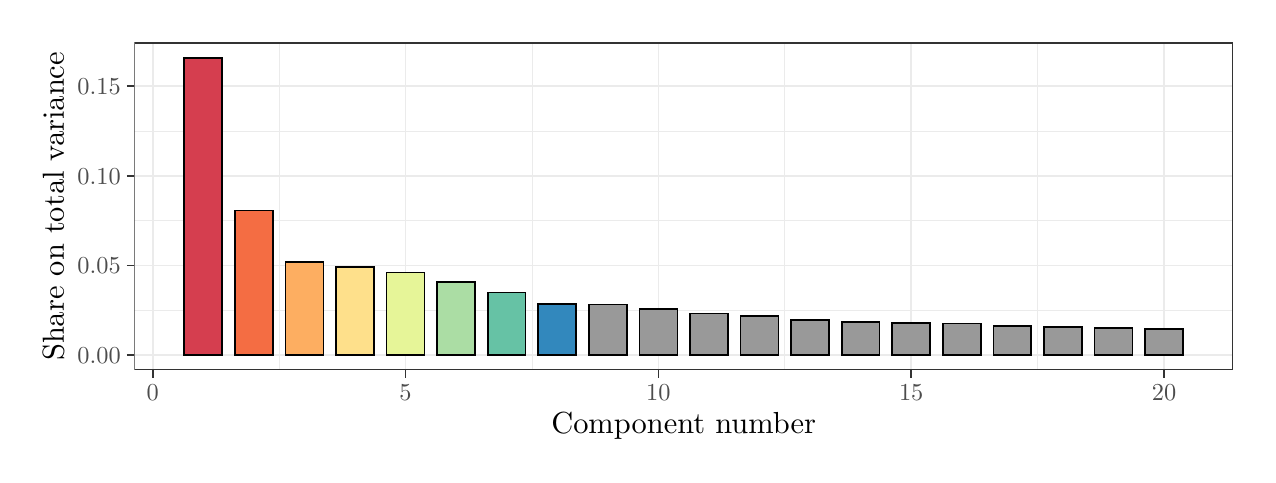
\begin{tikzpicture}[x=1pt,y=1pt]
\definecolor{fillColor}{RGB}{255,255,255}
\path[use as bounding box,fill=fillColor,fill opacity=0.00] (0,0) rectangle (441.02,154.36);
\begin{scope}
\path[clip] (  0.00,  0.00) rectangle (441.02,154.36);
\definecolor{drawColor}{RGB}{255,255,255}
\definecolor{fillColor}{RGB}{255,255,255}

\path[draw=drawColor,line width= 0.6pt,line join=round,line cap=round,fill=fillColor] (  0.00,  0.00) rectangle (441.02,154.36);
\end{scope}
\begin{scope}
\path[clip] ( 38.56, 30.69) rectangle (435.52,148.86);
\definecolor{fillColor}{RGB}{255,255,255}

\path[fill=fillColor] ( 38.56, 30.69) rectangle (435.52,148.86);
\definecolor{drawColor}{gray}{0.92}

\path[draw=drawColor,line width= 0.3pt,line join=round] ( 38.56, 52.24) --
	(435.52, 52.24);

\path[draw=drawColor,line width= 0.3pt,line join=round] ( 38.56, 84.61) --
	(435.52, 84.61);

\path[draw=drawColor,line width= 0.3pt,line join=round] ( 38.56,116.98) --
	(435.52,116.98);

\path[draw=drawColor,line width= 0.3pt,line join=round] ( 90.86, 30.69) --
	( 90.86,148.86);

\path[draw=drawColor,line width= 0.3pt,line join=round] (182.22, 30.69) --
	(182.22,148.86);

\path[draw=drawColor,line width= 0.3pt,line join=round] (273.58, 30.69) --
	(273.58,148.86);

\path[draw=drawColor,line width= 0.3pt,line join=round] (364.94, 30.69) --
	(364.94,148.86);

\path[draw=drawColor,line width= 0.6pt,line join=round] ( 38.56, 36.06) --
	(435.52, 36.06);

\path[draw=drawColor,line width= 0.6pt,line join=round] ( 38.56, 68.43) --
	(435.52, 68.43);

\path[draw=drawColor,line width= 0.6pt,line join=round] ( 38.56,100.80) --
	(435.52,100.80);

\path[draw=drawColor,line width= 0.6pt,line join=round] ( 38.56,133.17) --
	(435.52,133.17);

\path[draw=drawColor,line width= 0.6pt,line join=round] ( 45.18, 30.69) --
	( 45.18,148.86);

\path[draw=drawColor,line width= 0.6pt,line join=round] (136.54, 30.69) --
	(136.54,148.86);

\path[draw=drawColor,line width= 0.6pt,line join=round] (227.90, 30.69) --
	(227.90,148.86);

\path[draw=drawColor,line width= 0.6pt,line join=round] (319.26, 30.69) --
	(319.26,148.86);

\path[draw=drawColor,line width= 0.6pt,line join=round] (410.62, 30.69) --
	(410.62,148.86);
\definecolor{drawColor}{RGB}{0,0,0}
\definecolor{fillColor}{RGB}{213,62,79}

\path[draw=drawColor,line width= 0.6pt,line cap=rect,fill=fillColor] ( 56.60, 36.06) rectangle ( 70.30,143.48);
\definecolor{fillColor}{RGB}{244,109,67}

\path[draw=drawColor,line width= 0.6pt,line cap=rect,fill=fillColor] ( 74.87, 36.06) rectangle ( 88.58, 88.35);
\definecolor{fillColor}{RGB}{253,174,97}

\path[draw=drawColor,line width= 0.6pt,line cap=rect,fill=fillColor] ( 93.14, 36.06) rectangle (106.85, 69.74);
\definecolor{fillColor}{RGB}{254,224,139}

\path[draw=drawColor,line width= 0.6pt,line cap=rect,fill=fillColor] (111.42, 36.06) rectangle (125.12, 67.89);
\definecolor{fillColor}{RGB}{230,245,152}

\path[draw=drawColor,line width= 0.6pt,line cap=rect,fill=fillColor] (129.69, 36.06) rectangle (143.39, 65.91);
\definecolor{fillColor}{RGB}{171,221,164}

\path[draw=drawColor,line width= 0.6pt,line cap=rect,fill=fillColor] (147.96, 36.06) rectangle (161.66, 62.35);
\definecolor{fillColor}{RGB}{102,194,165}

\path[draw=drawColor,line width= 0.6pt,line cap=rect,fill=fillColor] (166.23, 36.06) rectangle (179.94, 58.68);
\definecolor{fillColor}{RGB}{50,136,189}

\path[draw=drawColor,line width= 0.6pt,line cap=rect,fill=fillColor] (184.50, 36.06) rectangle (198.21, 54.46);
\definecolor{fillColor}{gray}{0.60}

\path[draw=drawColor,line width= 0.6pt,line cap=rect,fill=fillColor] (202.78, 36.06) rectangle (216.48, 54.37);

\path[draw=drawColor,line width= 0.6pt,line cap=rect,fill=fillColor] (221.05, 36.06) rectangle (234.75, 52.69);

\path[draw=drawColor,line width= 0.6pt,line cap=rect,fill=fillColor] (239.32, 36.06) rectangle (253.02, 51.05);

\path[draw=drawColor,line width= 0.6pt,line cap=rect,fill=fillColor] (257.59, 36.06) rectangle (271.30, 50.25);

\path[draw=drawColor,line width= 0.6pt,line cap=rect,fill=fillColor] (275.86, 36.06) rectangle (289.57, 48.82);

\path[draw=drawColor,line width= 0.6pt,line cap=rect,fill=fillColor] (294.14, 36.06) rectangle (307.84, 47.90);

\path[draw=drawColor,line width= 0.6pt,line cap=rect,fill=fillColor] (312.41, 36.06) rectangle (326.11, 47.62);

\path[draw=drawColor,line width= 0.6pt,line cap=rect,fill=fillColor] (330.68, 36.06) rectangle (344.39, 47.44);

\path[draw=drawColor,line width= 0.6pt,line cap=rect,fill=fillColor] (348.95, 36.06) rectangle (362.66, 46.46);

\path[draw=drawColor,line width= 0.6pt,line cap=rect,fill=fillColor] (367.23, 36.06) rectangle (380.93, 46.27);

\path[draw=drawColor,line width= 0.6pt,line cap=rect,fill=fillColor] (385.50, 36.06) rectangle (399.20, 45.77);

\path[draw=drawColor,line width= 0.6pt,line cap=rect,fill=fillColor] (403.77, 36.06) rectangle (417.47, 45.58);
\definecolor{drawColor}{gray}{0.20}

\path[draw=drawColor,line width= 0.6pt,line join=round,line cap=round] ( 38.56, 30.69) rectangle (435.52,148.86);
\end{scope}
\begin{scope}
\path[clip] (  0.00,  0.00) rectangle (441.02,154.36);
\definecolor{drawColor}{gray}{0.30}

\node[text=drawColor,anchor=base east,inner sep=0pt, outer sep=0pt, scale=  0.88] at ( 33.61, 33.03) {0.00};

\node[text=drawColor,anchor=base east,inner sep=0pt, outer sep=0pt, scale=  0.88] at ( 33.61, 65.40) {0.05};

\node[text=drawColor,anchor=base east,inner sep=0pt, outer sep=0pt, scale=  0.88] at ( 33.61, 97.77) {0.10};

\node[text=drawColor,anchor=base east,inner sep=0pt, outer sep=0pt, scale=  0.88] at ( 33.61,130.14) {0.15};
\end{scope}
\begin{scope}
\path[clip] (  0.00,  0.00) rectangle (441.02,154.36);
\definecolor{drawColor}{gray}{0.20}

\path[draw=drawColor,line width= 0.6pt,line join=round] ( 35.81, 36.06) --
	( 38.56, 36.06);

\path[draw=drawColor,line width= 0.6pt,line join=round] ( 35.81, 68.43) --
	( 38.56, 68.43);

\path[draw=drawColor,line width= 0.6pt,line join=round] ( 35.81,100.80) --
	( 38.56,100.80);

\path[draw=drawColor,line width= 0.6pt,line join=round] ( 35.81,133.17) --
	( 38.56,133.17);
\end{scope}
\begin{scope}
\path[clip] (  0.00,  0.00) rectangle (441.02,154.36);
\definecolor{drawColor}{gray}{0.20}

\path[draw=drawColor,line width= 0.6pt,line join=round] ( 45.18, 27.94) --
	( 45.18, 30.69);

\path[draw=drawColor,line width= 0.6pt,line join=round] (136.54, 27.94) --
	(136.54, 30.69);

\path[draw=drawColor,line width= 0.6pt,line join=round] (227.90, 27.94) --
	(227.90, 30.69);

\path[draw=drawColor,line width= 0.6pt,line join=round] (319.26, 27.94) --
	(319.26, 30.69);

\path[draw=drawColor,line width= 0.6pt,line join=round] (410.62, 27.94) --
	(410.62, 30.69);
\end{scope}
\begin{scope}
\path[clip] (  0.00,  0.00) rectangle (441.02,154.36);
\definecolor{drawColor}{gray}{0.30}

\node[text=drawColor,anchor=base,inner sep=0pt, outer sep=0pt, scale=  0.88] at ( 45.18, 19.68) {0};

\node[text=drawColor,anchor=base,inner sep=0pt, outer sep=0pt, scale=  0.88] at (136.54, 19.68) {5};

\node[text=drawColor,anchor=base,inner sep=0pt, outer sep=0pt, scale=  0.88] at (227.90, 19.68) {10};

\node[text=drawColor,anchor=base,inner sep=0pt, outer sep=0pt, scale=  0.88] at (319.26, 19.68) {15};

\node[text=drawColor,anchor=base,inner sep=0pt, outer sep=0pt, scale=  0.88] at (410.62, 19.68) {20};
\end{scope}
\begin{scope}
\path[clip] (  0.00,  0.00) rectangle (441.02,154.36);
\definecolor{drawColor}{RGB}{0,0,0}

\node[text=drawColor,anchor=base,inner sep=0pt, outer sep=0pt, scale=  1.10] at (237.04,  7.64) {Component number};
\end{scope}
\begin{scope}
\path[clip] (  0.00,  0.00) rectangle (441.02,154.36);
\definecolor{drawColor}{RGB}{0,0,0}

\node[text=drawColor,rotate= 90.00,anchor=base,inner sep=0pt, outer sep=0pt, scale=  1.10] at ( 13.08, 89.77) {Share on total variance};
\end{scope}
\end{tikzpicture}
}
	\label{fig:Scree}
\end{figure}
In the resulting plot of Figure~\ref{fig:Scree}, the first eight eigenvalues for the relevant components are colored.\footnote{The vector graphics in this Latex document have been generated by the \pkg{tikzDevice} package \citep{SharpsteenEtAl2020}, which prints \proglang{R} plots as a Ti\textit{k}Z environment into ``.tex'' files.} They still account for almost 50\% of the total variation in the first-differenced and centered $K \cdot N$ time series, but the PCA of the original data attributes over $ 98\% $ to the first principal component alone. It appears that this all-dominating component is a linear trend in the time series, which is removed after first-differencing and centering. Now, the eighth and ninth eigenvalue are inconsiderable, while the first two exhibit more pronounced kinks. Indeed, the \textit{eigenvalue ratios} \code{ER} and \textit{growth rates} \code{GR} by \citet{AhnHorenstein2013} as well as \code{ED} by \citet{Onatski2010} hint at one resp.~two common factors.
\begin{CodeChunk}
\begin{CodeInput}		
R> R.fac0$selection[[2]]
\end{CodeInput}
\begin{CodeOutput}
ER GR ED 
1  1  2 
\end{CodeOutput}
\end{CodeChunk}
For the reproduction, we yet proceed with the decision by \citet{ArsovaOersal2017} and adhere to the conservative choice of eight common factors in order to ensure cross-sectional independence for the panel test.


\textbf{Panel cointegration tests.} The approximate factor model with \code{n.factors=8} yields a non-stationary,\footnote{Note that \citeauthor{Bronder2016}'s \citeyearpar{Bronder2016} \proglang{R}-package \pkg{PANICr} for single-equation PANIC methods, i.e.~unit root and residual-based cointegration tests, has been removed from CRAN lately. The methods rely on the same estimator for the common factors, that is a principal component analysis on the first-differenced variables, where the deterministic component has been removed. Consequently, the auxiliary function \code{aux\_ComFact()} can also be used for constructing own functions for these single-equation methods.} idiosyncratic remainder $ \boldsymbol{\hat{y}}^{i \! d}_{it} $, to which \citet{ArsovaOersal2017} apply the panel SL-tests. To reproduce their results, we specify \pkg{pvars}' function \code{pcoint.SL()} as follows. Due to the defactoring and in accordance with the econometric Model~\eqref{eq:MERM}, the $ N=19 $ individual testing procedures therein must take care of deterministic trends. The lag order $ p_i $ of each idiosyncratic VAR model is chosen from the discrete interval $ \lbrace 1,\ldots,4 \rbrace $ by the minimized \textit{Akaike information criterion}. Here, we enter the results directly, but \pkg{vars} functions may determine them from the data matrices in \code{R.fac0\$L.idio}, too.
\begin{CodeChunk}
\begin{CodeInput}
R> R.lags = c(2, 2, 2, 2, 1, 2, 2, 4, 2, 3, 2, 2, 2, 2, 2, 1, 1, 2, 2)
R> R.pcsl = pcoint.SL(L.data, lags=R.lags, type="SL_trend", n.factors=8)
R> toLatex(R.pcsl)
\end{CodeInput}
\end{CodeChunk}
The method \code{toLatex()} prints the \code{pcoint} results as a \code{tabular} for Latex, which has been encapsulated in Latex' float environment in order to create Table~\ref{tab:MERM}. 
\begin{table}[ht]	% tab:MERM
	\centering
	\caption[Cointegration rank tests]{Panel cointegration rank tests for MERM.} 
	\resizebox{0.8\textwidth}{!}{
		\begin{tabular}{lrrrrrrrrrr}
	\hline \hline
	\multicolumn{2}{l}{ \textbf{Individual} } & \multicolumn{4}{c}{ statistics } &  & \multicolumn{4}{c}{ $ p $-values } \\
	\cline{3-6} \cline{8-11}
	\multicolumn{2}{r}{ lags } & $ r_{H0} = 0 $ & $ r_{H0} = 1 $ & $ r_{H0} = 2 $ & $ r_{H0} = 3 $ &   & $ r_{H0} = 0 $ & $ r_{H0} = 1 $ & $ r_{H0} = 2 $ & $ r_{H0} = 3 $ \\
	\hline
	Brazil & 2 & 41.606 & 13.963 &  8.660 &  3.618 &   & 0.115 & 0.832 & 0.473 & 0.256 \\
	Canada & 2 & 43.889 & 19.816 &  6.253 &  0.413 &   & 0.070 & 0.406 & 0.747 & 0.940 \\
	Colombia & 2 & 25.210 & 13.042 &  4.744 &  1.914 &   & 0.875 & 0.881 & 0.891 & 0.558 \\
	Czech Republic & 2 & 29.238 & 17.663 &  7.712 &  0.583 &   & 0.689 & 0.568 & 0.580 & 0.901 \\
	Denmark & 1 & 37.925 & 18.804 &  7.758 &  2.450 &   & 0.230 & 0.480 & 0.575 & 0.442 \\
	Hungary & 2 & 32.372 & 16.940 &  8.401 &  0.863 &   & 0.510 & 0.624 & 0.502 & 0.829 \\
	India & 2 & 24.846 & 14.801 &  6.280 &  1.889 &   & 0.887 & 0.780 & 0.744 & 0.564 \\
	Indonesia & 4 & 26.911 & 12.640 &  4.211 &  1.687 &   & 0.806 & 0.899 & 0.928 & 0.612 \\
	Israel & 2 & 36.282 & 21.678 &  6.217 &  0.561 &   & 0.301 & 0.285 & 0.751 & 0.906 \\
	Japan & 3 & 28.154 & 15.395 &  6.966 &  1.975 &   & 0.746 & 0.739 & 0.667 & 0.544 \\
	Korea & 2 & 57.469 & 13.816 &  7.835 &  2.817 &   & 0.002 & 0.840 & 0.566 & 0.374 \\
	Mexico & 2 & 28.996 & 20.596 &  6.638 &  0.682 &   & 0.702 & 0.352 & 0.704 & 0.876 \\
	Norway & 2 & 43.766 & 19.633 &  6.715 &  1.367 &   & 0.072 & 0.419 & 0.696 & 0.694 \\
	Poland & 2 & 60.457 & 28.641 &  6.618 &  0.557 &   & 0.001 & 0.048 & 0.707 & 0.907 \\
	South Africa & 2 & 21.298 & 10.053 &  6.868 &  4.730 &   & 0.968 & 0.976 & 0.678 & 0.147 \\
	Sweden & 1 & 32.127 &  7.147 &  3.386 &  0.777 &   & 0.524 & 0.998 & 0.969 & 0.851 \\
	Switzerland & 1 & 28.419 & 13.682 &  3.413 &  1.699 &   & 0.733 & 0.848 & 0.968 & 0.609 \\
	Turkey & 2 & 48.692 & 27.137 & 14.041 &  0.325 &   & 0.021 & 0.075 & 0.094 & 0.958 \\
	United Kingdom & 2 & 50.253 & 24.440 &  4.287 &  3.031 &   & 0.014 & 0.152 & 0.923 & 0.339 \\
	 \hline
	\multicolumn{2}{l}{ \textbf{Panel} } & \multicolumn{4}{c}{ statistics } &  & \multicolumn{4}{c}{ $ p $-values } \\
	\cline{3-6} \cline{8-11}
	  &   & $ r_{H0} = 0 $ & $ r_{H0} = 1 $ & $ r_{H0} = 2 $ & $ r_{H0} = 3 $ &   & $ r_{H0} = 0 $ & $ r_{H0} = 1 $ & $ r_{H0} = 2 $ & $ r_{H0} = 3 $ \\
	\hline
	\multicolumn{2}{l}{LRbar} &  2.305 & -1.346 & -2.635 & -2.095 &   & 0.011 & 0.911 & 0.996 & 0.982 \\
	\multicolumn{2}{l}{Choi $P$} & 70.515 & 29.377 & 17.050 & 20.338 &   & 0.001 & 0.841 & 0.999 & 0.992 \\
	\multicolumn{2}{l}{Choi $Pm$} &  3.730 & -0.989 & -2.403 & -2.026 &   & 0.000 & 0.839 & 0.992 & 0.979 \\
	\multicolumn{2}{l}{Choi $Z$} & -1.914 &  1.528 &  2.639 &  2.124 &   & 0.028 & 0.937 & 0.996 & 0.983 \\
	\hline \hline
\end{tabular}
}	
	\label{tab:MERM}
\end{table}
The table reports the individual and panel results for each hypothesis $ r_{H0} = 0, \ldots, K-1 $, which refer to Table~5 in \citet[p.~68]{ArsovaOersal2017}. All four combination approaches under the independence assumption of the idiosyncratic VAR processes have been used. Comparing the $p$-values to a significance level of $ \alpha = 5 \% $, all sequential panel test procedures reject the hypotheses up to $ r_{H0} = 1 $ and thus confirm the presence of a single cointegration relation in $ \boldsymbol{{y}}^{i \! d}_{it} $.


\textbf{Cointegration rank of the factors.} Having determined the idiosyncratic cointegration rank, the PANIC turns then to the cointegration within the eight common factors $ \boldsymbol{F}_{t} $. The \code{\$CSD}-slot of the \code{pcoint} object contains the estimates for the cross-sectional dependence and is identical for the PANIC analysis of any \code{pcoint} function. Therein, the eigenvalues of the PCA are stored in the vector \code{eigenvals} and the cumulated common factors in the matrix \code{Ft} of dimension \code{dim\_T} $ \times $ \code{n.factors}. These multivariate time series shall be plotted firstly to get an overview as in Figur~4 of \citet[p.~71]{ArsovaOersal2017}. For this, we define the factor matrix \code{Ft} as a \code{ts} object with the same specifications as the observed time series and use the related plotting method via \code{autoplot()}. The package \pkg{ggfortify} \citep{TangEtAl2016} provides a comprehensive set of unified methods for \pkg{ggplot2} graphics.
\begin{CodeChunk}
\begin{CodeInput}
R> library("ggfortify")
R> Ft = ts(R.pcsl$CSD$Ft, start=c(1995, 1), frequency=12)
R> autoplot(Ft, facets=FALSE, size=1.5) + theme_bw() + 
+     scale_color_brewer(palette="Spectral") +
+     labs(x=NULL, y=NULL, color="Factor", title=NULL)
\end{CodeInput}
\end{CodeChunk}
\begin{figure}[ht] % fig:Factors
	\centering
	\caption{Estimated common factors.}
	\resizebox{0.8\textwidth}{!}{
		% Created by tikzDevice version 0.12.3.1 on 2021-02-24 10:31:38
% !TEX encoding = UTF-8 Unicode
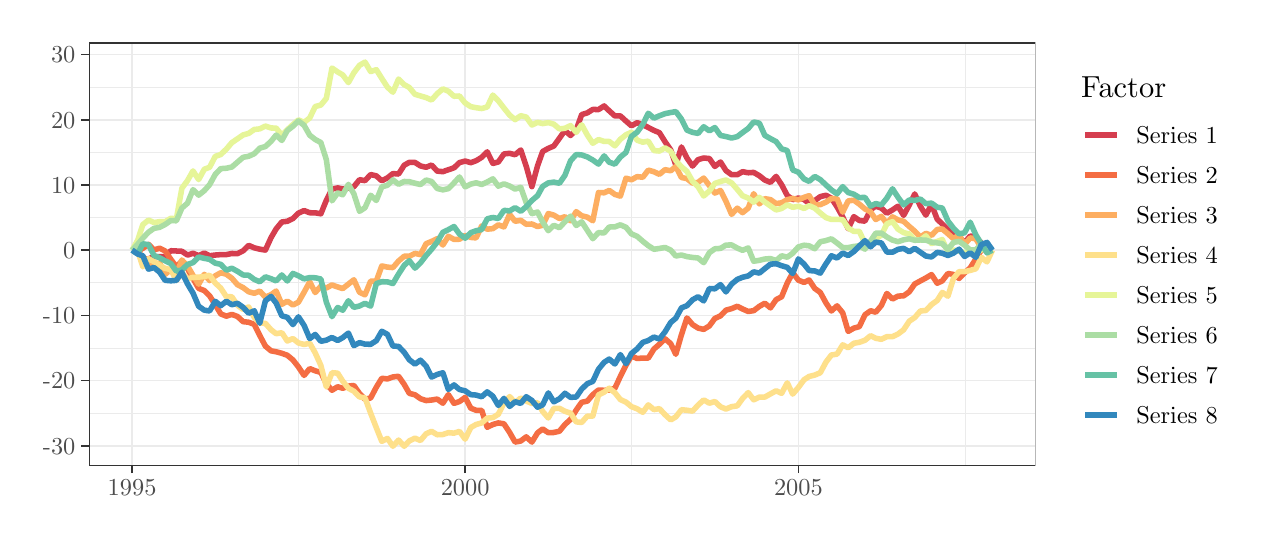
\begin{tikzpicture}[x=1pt,y=1pt]
\definecolor{fillColor}{RGB}{255,255,255}
\path[use as bounding box,fill=fillColor,fill opacity=0.00] (0,0) rectangle (441.02,176.41);
\begin{scope}
\path[clip] (  0.00,  0.00) rectangle (441.02,176.41);
\definecolor{drawColor}{RGB}{255,255,255}
\definecolor{fillColor}{RGB}{255,255,255}

\path[draw=drawColor,line width= 0.6pt,line join=round,line cap=round,fill=fillColor] (  0.00,  0.00) rectangle (441.02,176.41);
\end{scope}
\begin{scope}
\path[clip] ( 22.18, 18.22) rectangle (364.16,170.91);
\definecolor{fillColor}{RGB}{255,255,255}

\path[fill=fillColor] ( 22.18, 18.22) rectangle (364.16,170.91);
\definecolor{drawColor}{gray}{0.92}

\path[draw=drawColor,line width= 0.3pt,line join=round] ( 22.18, 37.12) --
	(364.16, 37.12);

\path[draw=drawColor,line width= 0.3pt,line join=round] ( 22.18, 60.68) --
	(364.16, 60.68);

\path[draw=drawColor,line width= 0.3pt,line join=round] ( 22.18, 84.23) --
	(364.16, 84.23);

\path[draw=drawColor,line width= 0.3pt,line join=round] ( 22.18,107.79) --
	(364.16,107.79);

\path[draw=drawColor,line width= 0.3pt,line join=round] ( 22.18,131.35) --
	(364.16,131.35);

\path[draw=drawColor,line width= 0.3pt,line join=round] ( 22.18,154.90) --
	(364.16,154.90);

\path[draw=drawColor,line width= 0.3pt,line join=round] ( 97.90, 18.22) --
	( 97.90,170.91);

\path[draw=drawColor,line width= 0.3pt,line join=round] (218.28, 18.22) --
	(218.28,170.91);

\path[draw=drawColor,line width= 0.3pt,line join=round] (338.67, 18.22) --
	(338.67,170.91);

\path[draw=drawColor,line width= 0.6pt,line join=round] ( 22.18, 25.34) --
	(364.16, 25.34);

\path[draw=drawColor,line width= 0.6pt,line join=round] ( 22.18, 48.90) --
	(364.16, 48.90);

\path[draw=drawColor,line width= 0.6pt,line join=round] ( 22.18, 72.46) --
	(364.16, 72.46);

\path[draw=drawColor,line width= 0.6pt,line join=round] ( 22.18, 96.01) --
	(364.16, 96.01);

\path[draw=drawColor,line width= 0.6pt,line join=round] ( 22.18,119.57) --
	(364.16,119.57);

\path[draw=drawColor,line width= 0.6pt,line join=round] ( 22.18,143.13) --
	(364.16,143.13);

\path[draw=drawColor,line width= 0.6pt,line join=round] ( 22.18,166.68) --
	(364.16,166.68);

\path[draw=drawColor,line width= 0.6pt,line join=round] ( 37.73, 18.22) --
	( 37.73,170.91);

\path[draw=drawColor,line width= 0.6pt,line join=round] (158.08, 18.22) --
	(158.08,170.91);

\path[draw=drawColor,line width= 0.6pt,line join=round] (278.49, 18.22) --
	(278.49,170.91);
\definecolor{drawColor}{RGB}{213,62,79}

\path[draw=drawColor,line width= 2.0pt,line join=round] ( 37.73, 96.01) --
	( 39.77, 95.28) --
	( 41.61, 92.97) --
	( 43.66, 92.85) --
	( 45.63, 93.68) --
	( 47.68, 93.71) --
	( 49.65, 93.67) --
	( 51.70, 95.81) --
	( 53.74, 95.71) --
	( 55.72, 95.61) --
	( 57.76, 94.23) --
	( 59.74, 94.89) --
	( 61.78, 94.04) --
	( 63.83, 94.97) --
	( 65.74, 94.01) --
	( 67.78, 94.25) --
	( 69.76, 94.40) --
	( 71.80, 94.42) --
	( 73.78, 94.81) --
	( 75.82, 94.76) --
	( 77.86, 95.79) --
	( 79.84, 97.75) --
	( 81.88, 96.86) --
	( 83.86, 96.37) --
	( 85.90, 96.04) --
	( 87.95,100.55) --
	( 89.79,103.71) --
	( 91.84,106.20) --
	( 93.81,106.45) --
	( 95.86,107.45) --
	( 97.83,109.38) --
	( 99.88,110.32) --
	(101.92,109.53) --
	(103.90,109.51) --
	(105.94,109.15) --
	(107.92,114.04) --
	(109.96,118.09) --
	(112.01,118.51) --
	(113.85,118.15) --
	(115.89,118.41) --
	(117.87,118.95) --
	(119.91,121.48) --
	(121.89,121.14) --
	(123.93,123.33) --
	(125.98,122.87) --
	(127.96,121.08) --
	(130.00,122.13) --
	(131.98,123.69) --
	(134.02,123.52) --
	(136.06,126.71) --
	(137.91,127.75) --
	(139.95,127.71) --
	(141.93,126.45) --
	(143.97,125.96) --
	(145.95,126.77) --
	(147.99,124.58) --
	(150.03,124.38) --
	(152.01,125.07) --
	(154.06,125.77) --
	(156.03,127.65) --
	(158.08,128.21) --
	(160.12,127.63) --
	(162.03,128.32) --
	(164.07,129.56) --
	(166.05,131.55) --
	(168.09,127.37) --
	(170.07,127.87) --
	(172.11,130.79) --
	(174.16,131.00) --
	(176.13,130.51) --
	(178.18,132.22) --
	(180.16,126.32) --
	(182.20,118.97) --
	(184.24,126.48) --
	(186.09,131.66) --
	(188.13,132.79) --
	(190.11,133.64) --
	(192.15,136.45) --
	(194.13,139.25) --
	(196.17,137.44) --
	(198.21,139.47) --
	(200.19,145.01) --
	(202.23,145.62) --
	(204.21,146.87) --
	(206.26,146.81) --
	(208.30,148.12) --
	(210.14,146.36) --
	(212.19,144.51) --
	(214.16,144.53) --
	(216.21,142.65) --
	(218.18,140.94) --
	(220.23,142.09) --
	(222.27,141.36) --
	(224.25,140.34) --
	(226.29,139.28) --
	(228.27,138.47) --
	(230.31,135.19) --
	(232.36,132.24) --
	(234.20,126.78) --
	(236.24,133.31) --
	(238.22,129.30) --
	(240.26,126.40) --
	(242.24,128.72) --
	(244.28,129.32) --
	(246.33,129.12) --
	(248.31,126.26) --
	(250.35,127.87) --
	(252.33,124.75) --
	(254.37,123.27) --
	(256.41,123.27) --
	(258.32,124.37) --
	(260.37,123.98) --
	(262.34,124.11) --
	(264.39,122.91) --
	(266.36,121.34) --
	(268.41,120.51) --
	(270.45,122.66) --
	(272.43,119.67) --
	(274.47,115.77) --
	(276.45,114.27) --
	(278.49,114.85) --
	(280.54,114.31) --
	(282.38,112.89) --
	(284.42,113.93) --
	(286.40,115.35) --
	(288.44,115.85) --
	(290.42,114.81) --
	(292.46,111.67) --
	(294.51,108.01) --
	(296.49,103.76) --
	(298.53,108.13) --
	(300.51,106.74) --
	(302.55,106.50) --
	(304.59,110.65) --
	(306.44,111.91) --
	(308.48,111.23) --
	(310.46,109.38) --
	(312.50,110.55) --
	(314.48,111.89) --
	(316.52,108.58) --
	(318.56,112.32) --
	(320.54,116.33) --
	(322.59,111.85) --
	(324.56,108.66) --
	(326.61,112.51) --
	(328.65,107.21) --
	(330.49,105.46) --
	(332.54,103.39) --
	(334.51,101.84) --
	(336.56,100.99) --
	(338.54, 98.69) --
	(340.58,101.14) --
	(342.62,100.65) --
	(344.60, 98.60) --
	(346.64, 95.51) --
	(348.62, 96.01);
\definecolor{drawColor}{RGB}{244,109,67}

\path[draw=drawColor,line width= 2.0pt,line join=round] ( 37.73, 96.01) --
	( 39.77, 95.71) --
	( 41.61, 96.67) --
	( 43.66, 98.10) --
	( 45.63, 96.11) --
	( 47.68, 96.71) --
	( 49.65, 95.75) --
	( 51.70, 92.74) --
	( 53.74, 89.99) --
	( 55.72, 92.03) --
	( 57.76, 89.33) --
	( 59.74, 85.75) --
	( 61.78, 82.21) --
	( 63.83, 81.40) --
	( 65.74, 79.53) --
	( 67.78, 76.27) --
	( 69.76, 72.98) --
	( 71.80, 72.16) --
	( 73.78, 72.80) --
	( 75.82, 72.04) --
	( 77.86, 70.17) --
	( 79.84, 69.97) --
	( 81.88, 69.19) --
	( 83.86, 65.21) --
	( 85.90, 61.34) --
	( 87.95, 59.63) --
	( 89.79, 59.30) --
	( 91.84, 58.74) --
	( 93.81, 58.03) --
	( 95.86, 56.34) --
	( 97.83, 53.83) --
	( 99.88, 50.76) --
	(101.92, 53.21) --
	(103.90, 52.42) --
	(105.94, 51.83) --
	(107.92, 47.75) --
	(109.96, 45.39) --
	(112.01, 46.66) --
	(113.85, 46.10) --
	(115.89, 46.90) --
	(117.87, 47.11) --
	(119.91, 44.22) --
	(121.89, 42.16) --
	(123.93, 42.60) --
	(125.98, 46.50) --
	(127.96, 49.72) --
	(130.00, 49.49) --
	(131.98, 50.20) --
	(134.02, 50.44) --
	(136.06, 47.51) --
	(137.91, 44.27) --
	(139.95, 43.75) --
	(141.93, 42.35) --
	(143.97, 41.66) --
	(145.95, 41.86) --
	(147.99, 42.20) --
	(150.03, 40.71) --
	(152.01, 43.81) --
	(154.06, 40.65) --
	(156.03, 41.31) --
	(158.08, 42.80) --
	(160.12, 38.92) --
	(162.03, 38.16) --
	(164.07, 38.13) --
	(166.05, 32.01) --
	(168.09, 33.02) --
	(170.07, 33.59) --
	(172.11, 33.26) --
	(174.16, 30.13) --
	(176.13, 26.66) --
	(178.18, 27.05) --
	(180.16, 28.55) --
	(182.20, 26.66) --
	(184.24, 30.00) --
	(186.09, 31.40) --
	(188.13, 30.05) --
	(190.11, 30.13) --
	(192.15, 30.59) --
	(194.13, 33.01) --
	(196.17, 34.87) --
	(198.21, 38.23) --
	(200.19, 41.04) --
	(202.23, 41.47) --
	(204.21, 43.82) --
	(206.26, 45.47) --
	(208.30, 45.37) --
	(210.14, 45.48) --
	(212.19, 46.12) --
	(214.16, 50.38) --
	(216.21, 54.47) --
	(218.18, 57.77) --
	(220.23, 56.87) --
	(222.27, 57.03) --
	(224.25, 57.00) --
	(226.29, 60.28) --
	(228.27, 62.01) --
	(230.31, 63.99) --
	(232.36, 62.23) --
	(234.20, 58.38) --
	(236.24, 65.46) --
	(238.22, 71.52) --
	(240.26, 69.12) --
	(242.24, 67.86) --
	(244.28, 67.39) --
	(246.33, 68.65) --
	(248.31, 71.34) --
	(250.35, 72.28) --
	(252.33, 74.33) --
	(254.37, 74.89) --
	(256.41, 75.74) --
	(258.32, 74.76) --
	(260.37, 73.86) --
	(262.34, 74.15) --
	(264.39, 75.70) --
	(266.36, 76.84) --
	(268.41, 75.16) --
	(270.45, 78.13) --
	(272.43, 79.17) --
	(274.47, 84.14) --
	(276.45, 87.84) --
	(278.49, 85.17) --
	(280.54, 84.35) --
	(282.38, 85.23) --
	(284.42, 82.17) --
	(286.40, 80.74) --
	(288.44, 77.00) --
	(290.42, 74.03) --
	(292.46, 75.89) --
	(294.51, 73.37) --
	(296.49, 66.67) --
	(298.53, 67.83) --
	(300.51, 68.38) --
	(302.55, 72.65) --
	(304.59, 74.12) --
	(306.44, 73.59) --
	(308.48, 76.03) --
	(310.46, 80.37) --
	(312.50, 78.34) --
	(314.48, 79.41) --
	(316.52, 79.51) --
	(318.56, 80.96) --
	(320.54, 83.79) --
	(322.59, 84.91) --
	(324.56, 85.96) --
	(326.61, 87.19) --
	(328.65, 84.07) --
	(330.49, 84.92) --
	(332.54, 87.59) --
	(334.51, 87.23) --
	(336.56, 85.79) --
	(338.54, 87.79) --
	(340.58, 89.61) --
	(342.62, 92.84) --
	(344.60, 96.05) --
	(346.64, 96.94) --
	(348.62, 96.01);
\definecolor{drawColor}{RGB}{253,174,97}

\path[draw=drawColor,line width= 2.0pt,line join=round] ( 37.73, 96.01) --
	( 39.77, 95.56) --
	( 41.61, 93.71) --
	( 43.66, 91.17) --
	( 45.63, 90.85) --
	( 47.68, 91.33) --
	( 49.65, 87.24) --
	( 51.70, 89.02) --
	( 53.74, 87.43) --
	( 55.72, 92.47) --
	( 57.76, 90.29) --
	( 59.74, 86.90) --
	( 61.78, 83.71) --
	( 63.83, 87.29) --
	( 65.74, 85.02) --
	( 67.78, 86.73) --
	( 69.76, 87.86) --
	( 71.80, 87.31) --
	( 73.78, 85.87) --
	( 75.82, 83.52) --
	( 77.86, 82.47) --
	( 79.84, 80.98) --
	( 81.88, 80.43) --
	( 83.86, 81.23) --
	( 85.90, 79.03) --
	( 87.95, 79.92) --
	( 89.79, 81.25) --
	( 91.84, 76.44) --
	( 93.81, 77.59) --
	( 95.86, 76.19) --
	( 97.83, 77.20) --
	( 99.88, 80.82) --
	(101.92, 84.56) --
	(103.90, 80.70) --
	(105.94, 82.99) --
	(107.92, 82.33) --
	(109.96, 83.45) --
	(112.01, 82.71) --
	(113.85, 82.13) --
	(115.89, 83.74) --
	(117.87, 85.32) --
	(119.91, 80.79) --
	(121.89, 79.87) --
	(123.93, 84.83) --
	(125.98, 84.85) --
	(127.96, 90.31) --
	(130.00, 89.88) --
	(131.98, 89.72) --
	(134.02, 92.08) --
	(136.06, 93.82) --
	(137.91, 93.81) --
	(139.95, 94.85) --
	(141.93, 94.40) --
	(143.97, 98.36) --
	(145.95, 99.17) --
	(147.99,100.17) --
	(150.03, 97.88) --
	(152.01,101.03) --
	(154.06, 99.89) --
	(156.03, 99.97) --
	(158.08,101.34) --
	(160.12,100.62) --
	(162.03,100.44) --
	(164.07,104.78) --
	(166.05,103.60) --
	(168.09,103.79) --
	(170.07,105.16) --
	(172.11,104.41) --
	(174.16,108.94) --
	(176.13,106.44) --
	(178.18,106.80) --
	(180.16,105.37) --
	(182.20,105.47) --
	(184.24,104.55) --
	(186.09,105.00) --
	(188.13,109.24) --
	(190.11,108.68) --
	(192.15,107.45) --
	(194.13,108.08) --
	(196.17,106.62) --
	(198.21,109.94) --
	(200.19,108.44) --
	(202.23,107.94) --
	(204.21,106.63) --
	(206.26,116.85) --
	(208.30,116.74) --
	(210.14,117.60) --
	(212.19,116.16) --
	(214.16,115.54) --
	(216.21,122.03) --
	(218.18,121.43) --
	(220.23,122.59) --
	(222.27,122.35) --
	(224.25,124.94) --
	(226.29,124.36) --
	(228.27,123.41) --
	(230.31,125.10) --
	(232.36,124.70) --
	(234.20,126.24) --
	(236.24,122.27) --
	(238.22,121.86) --
	(240.26,120.24) --
	(242.24,120.51) --
	(244.28,122.06) --
	(246.33,119.36) --
	(248.31,116.64) --
	(250.35,117.59) --
	(252.33,113.66) --
	(254.37,108.95) --
	(256.41,111.18) --
	(258.32,109.57) --
	(260.37,111.21) --
	(262.34,116.43) --
	(264.39,112.74) --
	(266.36,114.62) --
	(268.41,114.27) --
	(270.45,112.83) --
	(272.43,113.13) --
	(274.47,114.26) --
	(276.45,114.72) --
	(278.49,114.16) --
	(280.54,115.10) --
	(282.38,115.71) --
	(284.42,112.36) --
	(286.40,112.46) --
	(288.44,113.36) --
	(290.42,114.68) --
	(292.46,114.66) --
	(294.51,109.74) --
	(296.49,113.81) --
	(298.53,114.07) --
	(300.51,112.64) --
	(302.55,110.90) --
	(304.59,109.85) --
	(306.44,107.08) --
	(308.48,108.25) --
	(310.46,105.64) --
	(312.50,108.04) --
	(314.48,106.96) --
	(316.52,106.44) --
	(318.56,104.58) --
	(320.54,102.88) --
	(322.59,100.76) --
	(324.56,102.09) --
	(326.61,101.35) --
	(328.65,103.50) --
	(330.49,103.68) --
	(332.54,101.94) --
	(334.51,100.18) --
	(336.56,101.46) --
	(338.54, 98.06) --
	(340.58,100.44) --
	(342.62,100.12) --
	(344.60, 96.76) --
	(346.64, 95.43) --
	(348.62, 96.01);
\definecolor{drawColor}{RGB}{254,224,139}

\path[draw=drawColor,line width= 2.0pt,line join=round] ( 37.73, 96.01) --
	( 39.77, 95.78) --
	( 41.61, 90.01) --
	( 43.66, 92.93) --
	( 45.63, 91.88) --
	( 47.68, 90.54) --
	( 49.65, 89.43) --
	( 51.70, 89.01) --
	( 53.74, 85.07) --
	( 55.72, 87.76) --
	( 57.76, 85.70) --
	( 59.74, 86.18) --
	( 61.78, 86.26) --
	( 63.83, 86.47) --
	( 65.74, 86.95) --
	( 67.78, 84.14) --
	( 69.76, 82.31) --
	( 71.80, 79.18) --
	( 73.78, 79.17) --
	( 75.82, 76.07) --
	( 77.86, 74.60) --
	( 79.84, 75.49) --
	( 81.88, 71.71) --
	( 83.86, 69.71) --
	( 85.90, 69.54) --
	( 87.95, 67.24) --
	( 89.79, 65.83) --
	( 91.84, 66.18) --
	( 93.81, 63.20) --
	( 95.86, 64.07) --
	( 97.83, 62.49) --
	( 99.88, 61.94) --
	(101.92, 62.39) --
	(103.90, 58.89) --
	(105.94, 54.36) --
	(107.92, 46.60) --
	(109.96, 51.73) --
	(112.01, 51.57) --
	(113.85, 48.68) --
	(115.89, 46.10) --
	(117.87, 45.05) --
	(119.91, 42.98) --
	(121.89, 42.66) --
	(123.93, 37.12) --
	(125.98, 31.86) --
	(127.96, 26.95) --
	(130.00, 27.98) --
	(131.98, 25.16) --
	(134.02, 27.39) --
	(136.06, 25.16) --
	(137.91, 27.10) --
	(139.95, 28.07) --
	(141.93, 27.22) --
	(143.97, 29.67) --
	(145.95, 30.54) --
	(147.99, 29.31) --
	(150.03, 29.40) --
	(152.01, 30.07) --
	(154.06, 29.89) --
	(156.03, 30.54) --
	(158.08, 27.72) --
	(160.12, 31.93) --
	(162.03, 33.01) --
	(164.07, 33.59) --
	(166.05, 35.31) --
	(168.09, 35.51) --
	(170.07, 36.72) --
	(172.11, 40.76) --
	(174.16, 43.10) --
	(176.13, 40.94) --
	(178.18, 42.59) --
	(180.16, 41.49) --
	(182.20, 40.63) --
	(184.24, 40.93) --
	(186.09, 37.72) --
	(188.13, 35.37) --
	(190.11, 38.83) --
	(192.15, 38.86) --
	(194.13, 37.79) --
	(196.17, 37.13) --
	(198.21, 33.96) --
	(200.19, 33.76) --
	(202.23, 36.06) --
	(204.21, 36.08) --
	(206.26, 43.70) --
	(208.30, 44.72) --
	(210.14, 46.13) --
	(212.19, 44.50) --
	(214.16, 42.03) --
	(216.21, 41.09) --
	(218.18, 39.47) --
	(220.23, 38.69) --
	(222.27, 37.43) --
	(224.25, 40.10) --
	(226.29, 38.39) --
	(228.27, 38.75) --
	(230.31, 36.56) --
	(232.36, 34.68) --
	(234.20, 35.77) --
	(236.24, 38.36) --
	(238.22, 38.16) --
	(240.26, 37.86) --
	(242.24, 40.01) --
	(244.28, 41.90) --
	(246.33, 40.72) --
	(248.31, 41.32) --
	(250.35, 39.41) --
	(252.33, 38.61) --
	(254.37, 39.46) --
	(256.41, 39.75) --
	(258.32, 42.41) --
	(260.37, 44.53) --
	(262.34, 41.94) --
	(264.39, 42.91) --
	(266.36, 42.92) --
	(268.41, 44.08) --
	(270.45, 45.20) --
	(272.43, 44.28) --
	(274.47, 48.06) --
	(276.45, 44.01) --
	(278.49, 46.40) --
	(280.54, 49.20) --
	(282.38, 50.37) --
	(284.42, 50.89) --
	(286.40, 51.71) --
	(288.44, 55.53) --
	(290.42, 58.14) --
	(292.46, 58.45) --
	(294.51, 61.81) --
	(296.49, 60.74) --
	(298.53, 62.38) --
	(300.51, 62.72) --
	(302.55, 63.45) --
	(304.59, 65.11) --
	(306.44, 64.18) --
	(308.48, 63.80) --
	(310.46, 64.75) --
	(312.50, 64.76) --
	(314.48, 65.70) --
	(316.52, 67.23) --
	(318.56, 70.34) --
	(320.54, 71.66) --
	(322.59, 74.04) --
	(324.56, 74.23) --
	(326.61, 76.36) --
	(328.65, 77.83) --
	(330.49, 80.74) --
	(332.54, 79.37) --
	(334.51, 85.79) --
	(336.56, 88.25) --
	(338.54, 88.26) --
	(340.58, 88.70) --
	(342.62, 89.28) --
	(344.60, 93.43) --
	(346.64, 91.79) --
	(348.62, 96.01);
\definecolor{drawColor}{RGB}{230,245,152}

\path[draw=drawColor,line width= 2.0pt,line join=round] ( 37.73, 96.01) --
	( 39.77, 99.64) --
	( 41.61,105.25) --
	( 43.66,106.88) --
	( 45.63,105.99) --
	( 47.68,106.31) --
	( 49.65,106.29) --
	( 51.70,107.52) --
	( 53.74,107.36) --
	( 55.72,118.37) --
	( 57.76,121.16) --
	( 59.74,124.64) --
	( 61.78,121.51) --
	( 63.83,125.25) --
	( 65.74,125.97) --
	( 67.78,129.90) --
	( 69.76,130.57) --
	( 71.80,132.54) --
	( 73.78,134.86) --
	( 75.82,136.26) --
	( 77.86,137.66) --
	( 79.84,138.20) --
	( 81.88,139.62) --
	( 83.86,139.84) --
	( 85.90,140.86) --
	( 87.95,140.16) --
	( 89.79,140.13) --
	( 91.84,137.54) --
	( 93.81,139.53) --
	( 95.86,141.42) --
	( 97.83,143.07) --
	( 99.88,142.20) --
	(101.92,143.77) --
	(103.90,147.91) --
	(105.94,148.45) --
	(107.92,150.86) --
	(109.96,161.82) --
	(112.01,160.40) --
	(113.85,159.35) --
	(115.89,156.56) --
	(117.87,160.13) --
	(119.91,162.80) --
	(121.89,163.97) --
	(123.93,160.54) --
	(125.98,161.24) --
	(127.96,158.07) --
	(130.00,154.91) --
	(131.98,153.09) --
	(134.02,157.86) --
	(136.06,155.82) --
	(137.91,154.78) --
	(139.95,152.33) --
	(141.93,151.74) --
	(143.97,151.14) --
	(145.95,150.27) --
	(147.99,152.57) --
	(150.03,154.29) --
	(152.01,153.44) --
	(154.06,151.62) --
	(156.03,151.72) --
	(158.08,149.18) --
	(160.12,147.86) --
	(162.03,147.49) --
	(164.07,147.19) --
	(166.05,147.74) --
	(168.09,152.05) --
	(170.07,150.00) --
	(172.11,147.36) --
	(174.16,144.81) --
	(176.13,143.18) --
	(178.18,144.61) --
	(180.16,144.10) --
	(182.20,141.22) --
	(184.24,142.21) --
	(186.09,141.76) --
	(188.13,142.10) --
	(190.11,141.55) --
	(192.15,139.81) --
	(194.13,140.05) --
	(196.17,141.03) --
	(198.21,138.56) --
	(200.19,141.31) --
	(202.23,137.60) --
	(204.21,134.65) --
	(206.26,135.97) --
	(208.30,135.32) --
	(210.14,135.28) --
	(212.19,133.72) --
	(214.16,136.08) --
	(216.21,137.72) --
	(218.18,138.63) --
	(220.23,135.73) --
	(222.27,135.03) --
	(224.25,135.41) --
	(226.29,132.00) --
	(228.27,131.83) --
	(230.31,132.98) --
	(232.36,131.75) --
	(234.20,128.38) --
	(236.24,126.12) --
	(238.22,124.47) --
	(240.26,120.90) --
	(242.24,118.95) --
	(244.28,115.58) --
	(246.33,117.40) --
	(248.31,120.12) --
	(250.35,120.82) --
	(252.33,121.38) --
	(254.37,120.31) --
	(256.41,117.98) --
	(258.32,115.66) --
	(260.37,114.83) --
	(262.34,113.37) --
	(264.39,115.09) --
	(266.36,113.42) --
	(268.41,111.97) --
	(270.45,110.55) --
	(272.43,111.07) --
	(274.47,112.40) --
	(276.45,111.50) --
	(278.49,111.89) --
	(280.54,111.08) --
	(282.38,112.08) --
	(284.42,111.18) --
	(286.40,109.45) --
	(288.44,107.78) --
	(290.42,107.13) --
	(292.46,107.14) --
	(294.51,107.06) --
	(296.49,104.02) --
	(298.53,102.79) --
	(300.51,102.83) --
	(302.55, 98.50) --
	(304.59, 98.76) --
	(306.44,100.20) --
	(308.48,101.43) --
	(310.46,105.53) --
	(312.50,106.33) --
	(314.48,103.61) --
	(316.52,102.34) --
	(318.56,101.86) --
	(320.54, 99.73) --
	(322.59, 99.66) --
	(324.56,101.19) --
	(326.61, 98.40) --
	(328.65, 99.15) --
	(330.49, 99.85) --
	(332.54, 95.27) --
	(334.51, 96.07) --
	(336.56, 95.69) --
	(338.54, 95.06) --
	(340.58, 94.85) --
	(342.62, 94.66) --
	(344.60, 96.21) --
	(346.64, 96.29) --
	(348.62, 96.01);
\definecolor{drawColor}{RGB}{171,221,164}

\path[draw=drawColor,line width= 2.0pt,line join=round] ( 37.73, 96.01) --
	( 39.77, 98.14) --
	( 41.61,100.36) --
	( 43.66,102.50) --
	( 45.63,103.89) --
	( 47.68,104.26) --
	( 49.65,105.27) --
	( 51.70,106.71) --
	( 53.74,106.63) --
	( 55.72,111.23) --
	( 57.76,112.99) --
	( 59.74,117.88) --
	( 61.78,115.89) --
	( 63.83,117.53) --
	( 65.74,119.67) --
	( 67.78,123.39) --
	( 69.76,125.47) --
	( 71.80,125.62) --
	( 73.78,126.05) --
	( 75.82,127.83) --
	( 77.86,129.57) --
	( 79.84,129.93) --
	( 81.88,130.87) --
	( 83.86,132.87) --
	( 85.90,133.46) --
	( 87.95,135.35) --
	( 89.79,137.61) --
	( 91.84,135.65) --
	( 93.81,139.22) --
	( 95.86,140.80) --
	( 97.83,142.69) --
	( 99.88,141.12) --
	(101.92,137.55) --
	(103.90,136.01) --
	(105.94,134.90) --
	(107.92,128.75) --
	(109.96,113.82) --
	(112.01,116.70) --
	(113.85,116.03) --
	(115.89,119.80) --
	(117.87,116.38) --
	(119.91,110.05) --
	(121.89,111.35) --
	(123.93,115.86) --
	(125.98,113.96) --
	(127.96,118.87) --
	(130.00,119.47) --
	(131.98,121.44) --
	(134.02,119.81) --
	(136.06,120.83) --
	(137.91,120.75) --
	(139.95,120.20) --
	(141.93,119.72) --
	(143.97,121.35) --
	(145.95,120.83) --
	(147.99,118.30) --
	(150.03,117.81) --
	(152.01,118.24) --
	(154.06,120.32) --
	(156.03,122.46) --
	(158.08,118.89) --
	(160.12,119.87) --
	(162.03,120.36) --
	(164.07,119.75) --
	(166.05,120.64) --
	(168.09,121.79) --
	(170.07,119.14) --
	(172.11,119.97) --
	(174.16,119.19) --
	(176.13,118.08) --
	(178.18,118.72) --
	(180.16,113.14) --
	(182.20,109.21) --
	(184.24,109.79) --
	(186.09,106.19) --
	(188.13,103.05) --
	(190.11,104.99) --
	(192.15,104.12) --
	(194.13,106.28) --
	(196.17,108.31) --
	(198.21,104.92) --
	(200.19,106.24) --
	(202.23,103.16) --
	(204.21,100.15) --
	(206.26,102.38) --
	(208.30,102.23) --
	(210.14,104.37) --
	(212.19,104.44) --
	(214.16,105.17) --
	(216.21,104.27) --
	(218.18,101.88) --
	(220.23,101.00) --
	(222.27, 99.23) --
	(224.25, 97.65) --
	(226.29, 96.33) --
	(228.27, 96.63) --
	(230.31, 96.98) --
	(232.36, 96.03) --
	(234.20, 93.89) --
	(236.24, 94.26) --
	(238.22, 93.69) --
	(240.26, 93.38) --
	(242.24, 93.18) --
	(244.28, 91.50) --
	(246.33, 95.10) --
	(248.31, 96.51) --
	(250.35, 96.65) --
	(252.33, 97.85) --
	(254.37, 97.90) --
	(256.41, 96.77) --
	(258.32, 95.95) --
	(260.37, 96.81) --
	(262.34, 92.01) --
	(264.39, 92.34) --
	(266.36, 92.81) --
	(268.41, 92.97) --
	(270.45, 92.26) --
	(272.43, 93.98) --
	(274.47, 93.47) --
	(276.45, 94.91) --
	(278.49, 97.18) --
	(280.54, 97.80) --
	(282.38, 97.58) --
	(284.42, 96.54) --
	(286.40, 99.04) --
	(288.44, 99.47) --
	(290.42,100.11) --
	(292.46, 98.60) --
	(294.51, 96.96) --
	(296.49, 96.93) --
	(298.53, 97.34) --
	(300.51, 97.61) --
	(302.55, 96.38) --
	(304.59, 99.35) --
	(306.44,102.16) --
	(308.48,102.19) --
	(310.46,100.78) --
	(312.50, 99.64) --
	(314.48, 99.08) --
	(316.52, 99.75) --
	(318.56,100.13) --
	(320.54, 99.58) --
	(322.59, 99.70) --
	(324.56, 99.63) --
	(326.61, 98.94) --
	(328.65, 98.64) --
	(330.49, 98.36) --
	(332.54, 96.29) --
	(334.51, 98.78) --
	(336.56, 99.21) --
	(338.54, 97.81) --
	(340.58, 96.08) --
	(342.62, 96.14) --
	(344.60, 98.31) --
	(346.64, 96.93) --
	(348.62, 96.01);
\definecolor{drawColor}{RGB}{102,194,165}

\path[draw=drawColor,line width= 2.0pt,line join=round] ( 37.73, 96.01) --
	( 39.77, 94.71) --
	( 41.61, 98.31) --
	( 43.66, 97.99) --
	( 45.63, 94.12) --
	( 47.68, 93.25) --
	( 49.65, 92.17) --
	( 51.70, 91.19) --
	( 53.74, 88.43) --
	( 55.72, 88.87) --
	( 57.76, 90.85) --
	( 59.74, 91.50) --
	( 61.78, 93.56) --
	( 63.83, 93.05) --
	( 65.74, 92.70) --
	( 67.78, 91.32) --
	( 69.76, 90.89) --
	( 71.80, 88.79) --
	( 73.78, 89.49) --
	( 75.82, 88.36) --
	( 77.86, 87.05) --
	( 79.84, 86.94) --
	( 81.88, 85.44) --
	( 83.86, 84.59) --
	( 85.90, 86.36) --
	( 87.95, 85.69) --
	( 89.79, 84.91) --
	( 91.84, 87.05) --
	( 93.81, 84.88) --
	( 95.86, 87.61) --
	( 97.83, 86.74) --
	( 99.88, 85.63) --
	(101.92, 86.10) --
	(103.90, 86.03) --
	(105.94, 85.60) --
	(107.92, 77.21) --
	(109.96, 71.99) --
	(112.01, 75.30) --
	(113.85, 74.30) --
	(115.89, 77.73) --
	(117.87, 75.35) --
	(119.91, 75.84) --
	(121.89, 76.81) --
	(123.93, 75.80) --
	(125.98, 83.93) --
	(127.96, 84.61) --
	(130.00, 84.56) --
	(131.98, 83.95) --
	(134.02, 87.38) --
	(136.06, 90.53) --
	(137.91, 92.20) --
	(139.95, 89.53) --
	(141.93, 91.43) --
	(143.97, 94.07) --
	(145.95, 96.34) --
	(147.99, 98.93) --
	(150.03,102.46) --
	(152.01,103.41) --
	(154.06,104.55) --
	(156.03,101.83) --
	(158.08,100.34) --
	(160.12,102.33) --
	(162.03,103.03) --
	(164.07,103.46) --
	(166.05,107.33) --
	(168.09,107.83) --
	(170.07,107.44) --
	(172.11,110.40) --
	(174.16,110.19) --
	(176.13,111.38) --
	(178.18,110.05) --
	(180.16,111.75) --
	(182.20,113.97) --
	(184.24,115.69) --
	(186.09,119.05) --
	(188.13,120.32) --
	(190.11,120.60) --
	(192.15,120.19) --
	(194.13,123.04) --
	(196.17,128.32) --
	(198.21,130.57) --
	(200.19,130.42) --
	(202.23,129.70) --
	(204.21,128.58) --
	(206.26,127.12) --
	(208.30,130.07) --
	(210.14,127.79) --
	(212.19,127.09) --
	(214.16,129.65) --
	(216.21,131.34) --
	(218.18,137.14) --
	(220.23,138.65) --
	(222.27,141.44) --
	(224.25,145.48) --
	(226.29,143.72) --
	(228.27,144.57) --
	(230.31,145.34) --
	(232.36,145.75) --
	(234.20,146.09) --
	(236.24,143.36) --
	(238.22,139.40) --
	(240.26,138.58) --
	(242.24,138.20) --
	(244.28,140.62) --
	(246.33,139.12) --
	(248.31,140.33) --
	(250.35,137.46) --
	(252.33,137.07) --
	(254.37,136.53) --
	(256.41,137.05) --
	(258.32,138.50) --
	(260.37,139.99) --
	(262.34,142.33) --
	(264.39,141.90) --
	(266.36,137.48) --
	(268.41,136.32) --
	(270.45,135.23) --
	(272.43,132.61) --
	(274.47,132.02) --
	(276.45,124.99) --
	(278.49,124.19) --
	(280.54,121.72) --
	(282.38,120.88) --
	(284.42,122.65) --
	(286.40,121.51) --
	(288.44,119.60) --
	(290.42,117.78) --
	(292.46,116.36) --
	(294.51,118.98) --
	(296.49,116.84) --
	(298.53,116.23) --
	(300.51,115.01) --
	(302.55,115.07) --
	(304.59,111.93) --
	(306.44,112.84) --
	(308.48,112.35) --
	(310.46,114.81) --
	(312.50,118.19) --
	(314.48,115.14) --
	(316.52,112.36) --
	(318.56,114.16) --
	(320.54,113.98) --
	(322.59,114.48) --
	(324.56,112.80) --
	(326.61,113.01) --
	(328.65,111.54) --
	(330.49,111.24) --
	(332.54,106.54) --
	(334.51,103.99) --
	(336.56,101.93) --
	(338.54,102.27) --
	(340.58,106.12) --
	(342.62,101.53) --
	(344.60, 98.33) --
	(346.64, 95.03) --
	(348.62, 96.01);
\definecolor{drawColor}{RGB}{50,136,189}

\path[draw=drawColor,line width= 2.0pt,line join=round] ( 37.73, 96.01) --
	( 39.77, 94.60) --
	( 41.61, 93.98) --
	( 43.66, 89.15) --
	( 45.63, 89.75) --
	( 47.68, 88.05) --
	( 49.65, 85.11) --
	( 51.70, 84.94) --
	( 53.74, 85.10) --
	( 55.72, 88.04) --
	( 57.76, 83.82) --
	( 59.74, 80.51) --
	( 61.78, 75.75) --
	( 63.83, 74.33) --
	( 65.74, 74.04) --
	( 67.78, 77.54) --
	( 69.76, 75.95) --
	( 71.80, 77.55) --
	( 73.78, 76.29) --
	( 75.82, 76.81) --
	( 77.86, 75.35) --
	( 79.84, 73.22) --
	( 81.88, 74.10) --
	( 83.86, 69.59) --
	( 85.90, 77.71) --
	( 87.95, 79.31) --
	( 89.79, 76.89) --
	( 91.84, 72.29) --
	( 93.81, 71.74) --
	( 95.86, 69.11) --
	( 97.83, 71.93) --
	( 99.88, 68.83) --
	(101.92, 64.05) --
	(103.90, 65.55) --
	(105.94, 63.08) --
	(107.92, 63.49) --
	(109.96, 64.46) --
	(112.01, 63.37) --
	(113.85, 64.41) --
	(115.89, 66.05) --
	(117.87, 61.51) --
	(119.91, 62.61) --
	(121.89, 62.06) --
	(123.93, 61.99) --
	(125.98, 63.29) --
	(127.96, 66.71) --
	(130.00, 65.59) --
	(131.98, 61.36) --
	(134.02, 61.24) --
	(136.06, 59.09) --
	(137.91, 56.40) --
	(139.95, 54.84) --
	(141.93, 56.25) --
	(143.97, 54.12) --
	(145.95, 50.15) --
	(147.99, 51.11) --
	(150.03, 51.71) --
	(152.01, 45.69) --
	(154.06, 47.32) --
	(156.03, 45.66) --
	(158.08, 45.18) --
	(160.12, 43.80) --
	(162.03, 43.65) --
	(164.07, 43.05) --
	(166.05, 44.81) --
	(168.09, 43.24) --
	(170.07, 39.89) --
	(172.11, 42.45) --
	(174.16, 39.56) --
	(176.13, 41.24) --
	(178.18, 40.64) --
	(180.16, 43.06) --
	(182.20, 41.69) --
	(184.24, 39.27) --
	(186.09, 40.12) --
	(188.13, 44.43) --
	(190.11, 41.21) --
	(192.15, 42.30) --
	(194.13, 44.31) --
	(196.17, 42.82) --
	(198.21, 42.94) --
	(200.19, 45.81) --
	(202.23, 47.77) --
	(204.21, 48.59) --
	(206.26, 52.98) --
	(208.30, 55.47) --
	(210.14, 56.66) --
	(212.19, 54.88) --
	(214.16, 58.28) --
	(216.21, 55.00) --
	(218.18, 58.68) --
	(220.23, 60.34) --
	(222.27, 62.68) --
	(224.25, 63.37) --
	(226.29, 64.62) --
	(228.27, 63.89) --
	(230.31, 66.50) --
	(232.36, 69.89) --
	(234.20, 71.43) --
	(236.24, 75.16) --
	(238.22, 75.94) --
	(240.26, 78.08) --
	(242.24, 79.18) --
	(244.28, 77.68) --
	(246.33, 82.16) --
	(248.31, 82.05) --
	(250.35, 83.56) --
	(252.33, 80.94) --
	(254.37, 83.76) --
	(256.41, 85.45) --
	(258.32, 86.22) --
	(260.37, 86.70) --
	(262.34, 88.17) --
	(264.39, 87.73) --
	(266.36, 89.34) --
	(268.41, 90.95) --
	(270.45, 91.12) --
	(272.43, 90.39) --
	(274.47, 89.80) --
	(276.45, 87.55) --
	(278.49, 92.86) --
	(280.54, 90.98) --
	(282.38, 88.63) --
	(284.42, 88.51) --
	(286.40, 87.71) --
	(288.44, 91.06) --
	(290.42, 93.99) --
	(292.46, 93.18) --
	(294.51, 94.97) --
	(296.49, 94.07) --
	(298.53, 95.50) --
	(300.51, 97.51) --
	(302.55, 99.46) --
	(304.59, 97.23) --
	(306.44, 98.93) --
	(308.48, 98.61) --
	(310.46, 95.35) --
	(312.50, 95.27) --
	(314.48, 96.31) --
	(316.52, 96.65) --
	(318.56, 95.44) --
	(320.54, 96.67) --
	(322.59, 95.25) --
	(324.56, 93.89) --
	(326.61, 93.55) --
	(328.65, 95.22) --
	(330.49, 94.90) --
	(332.54, 94.10) --
	(334.51, 94.94) --
	(336.56, 96.37) --
	(338.54, 93.73) --
	(340.58, 95.03) --
	(342.62, 93.42) --
	(344.60, 98.00) --
	(346.64, 98.82) --
	(348.62, 96.01);
\definecolor{drawColor}{gray}{0.20}

\path[draw=drawColor,line width= 0.6pt,line join=round,line cap=round] ( 22.18, 18.22) rectangle (364.16,170.91);
\end{scope}
\begin{scope}
\path[clip] (  0.00,  0.00) rectangle (441.02,176.41);
\definecolor{drawColor}{gray}{0.30}

\node[text=drawColor,anchor=base east,inner sep=0pt, outer sep=0pt, scale=  0.88] at ( 17.23, 22.31) {-30};

\node[text=drawColor,anchor=base east,inner sep=0pt, outer sep=0pt, scale=  0.88] at ( 17.23, 45.87) {-20};

\node[text=drawColor,anchor=base east,inner sep=0pt, outer sep=0pt, scale=  0.88] at ( 17.23, 69.43) {-10};

\node[text=drawColor,anchor=base east,inner sep=0pt, outer sep=0pt, scale=  0.88] at ( 17.23, 92.98) {0};

\node[text=drawColor,anchor=base east,inner sep=0pt, outer sep=0pt, scale=  0.88] at ( 17.23,116.54) {10};

\node[text=drawColor,anchor=base east,inner sep=0pt, outer sep=0pt, scale=  0.88] at ( 17.23,140.10) {20};

\node[text=drawColor,anchor=base east,inner sep=0pt, outer sep=0pt, scale=  0.88] at ( 17.23,163.65) {30};
\end{scope}
\begin{scope}
\path[clip] (  0.00,  0.00) rectangle (441.02,176.41);
\definecolor{drawColor}{gray}{0.20}

\path[draw=drawColor,line width= 0.6pt,line join=round] ( 19.43, 25.34) --
	( 22.18, 25.34);

\path[draw=drawColor,line width= 0.6pt,line join=round] ( 19.43, 48.90) --
	( 22.18, 48.90);

\path[draw=drawColor,line width= 0.6pt,line join=round] ( 19.43, 72.46) --
	( 22.18, 72.46);

\path[draw=drawColor,line width= 0.6pt,line join=round] ( 19.43, 96.01) --
	( 22.18, 96.01);

\path[draw=drawColor,line width= 0.6pt,line join=round] ( 19.43,119.57) --
	( 22.18,119.57);

\path[draw=drawColor,line width= 0.6pt,line join=round] ( 19.43,143.13) --
	( 22.18,143.13);

\path[draw=drawColor,line width= 0.6pt,line join=round] ( 19.43,166.68) --
	( 22.18,166.68);
\end{scope}
\begin{scope}
\path[clip] (  0.00,  0.00) rectangle (441.02,176.41);
\definecolor{drawColor}{gray}{0.20}

\path[draw=drawColor,line width= 0.6pt,line join=round] ( 37.73, 15.47) --
	( 37.73, 18.22);

\path[draw=drawColor,line width= 0.6pt,line join=round] (158.08, 15.47) --
	(158.08, 18.22);

\path[draw=drawColor,line width= 0.6pt,line join=round] (278.49, 15.47) --
	(278.49, 18.22);
\end{scope}
\begin{scope}
\path[clip] (  0.00,  0.00) rectangle (441.02,176.41);
\definecolor{drawColor}{gray}{0.30}

\node[text=drawColor,anchor=base,inner sep=0pt, outer sep=0pt, scale=  0.88] at ( 37.73,  7.21) {1995};

\node[text=drawColor,anchor=base,inner sep=0pt, outer sep=0pt, scale=  0.88] at (158.08,  7.21) {2000};

\node[text=drawColor,anchor=base,inner sep=0pt, outer sep=0pt, scale=  0.88] at (278.49,  7.21) {2005};
\end{scope}
\begin{scope}
\path[clip] (  0.00,  0.00) rectangle (441.02,176.41);
\definecolor{fillColor}{RGB}{255,255,255}

\path[fill=fillColor] (375.16, 23.64) rectangle (435.52,165.49);
\end{scope}
\begin{scope}
\path[clip] (  0.00,  0.00) rectangle (441.02,176.41);
\definecolor{drawColor}{RGB}{0,0,0}

\node[text=drawColor,anchor=base west,inner sep=0pt, outer sep=0pt, scale=  1.10] at (380.66,151.34) {Factor};
\end{scope}
\begin{scope}
\path[clip] (  0.00,  0.00) rectangle (441.02,176.41);
\definecolor{fillColor}{RGB}{255,255,255}

\path[fill=fillColor] (380.66,130.32) rectangle (395.12,144.77);
\end{scope}
\begin{scope}
\path[clip] (  0.00,  0.00) rectangle (441.02,176.41);
\definecolor{drawColor}{RGB}{213,62,79}

\path[draw=drawColor,line width= 2.0pt,line join=round] (382.11,137.55) -- (393.67,137.55);
\end{scope}
\begin{scope}
\path[clip] (  0.00,  0.00) rectangle (441.02,176.41);
\definecolor{fillColor}{RGB}{255,255,255}

\path[fill=fillColor] (380.66,115.87) rectangle (395.12,130.32);
\end{scope}
\begin{scope}
\path[clip] (  0.00,  0.00) rectangle (441.02,176.41);
\definecolor{drawColor}{RGB}{244,109,67}

\path[draw=drawColor,line width= 2.0pt,line join=round] (382.11,123.09) -- (393.67,123.09);
\end{scope}
\begin{scope}
\path[clip] (  0.00,  0.00) rectangle (441.02,176.41);
\definecolor{fillColor}{RGB}{255,255,255}

\path[fill=fillColor] (380.66,101.41) rectangle (395.12,115.87);
\end{scope}
\begin{scope}
\path[clip] (  0.00,  0.00) rectangle (441.02,176.41);
\definecolor{drawColor}{RGB}{253,174,97}

\path[draw=drawColor,line width= 2.0pt,line join=round] (382.11,108.64) -- (393.67,108.64);
\end{scope}
\begin{scope}
\path[clip] (  0.00,  0.00) rectangle (441.02,176.41);
\definecolor{fillColor}{RGB}{255,255,255}

\path[fill=fillColor] (380.66, 86.96) rectangle (395.12,101.41);
\end{scope}
\begin{scope}
\path[clip] (  0.00,  0.00) rectangle (441.02,176.41);
\definecolor{drawColor}{RGB}{254,224,139}

\path[draw=drawColor,line width= 2.0pt,line join=round] (382.11, 94.18) -- (393.67, 94.18);
\end{scope}
\begin{scope}
\path[clip] (  0.00,  0.00) rectangle (441.02,176.41);
\definecolor{fillColor}{RGB}{255,255,255}

\path[fill=fillColor] (380.66, 72.50) rectangle (395.12, 86.96);
\end{scope}
\begin{scope}
\path[clip] (  0.00,  0.00) rectangle (441.02,176.41);
\definecolor{drawColor}{RGB}{230,245,152}

\path[draw=drawColor,line width= 2.0pt,line join=round] (382.11, 79.73) -- (393.67, 79.73);
\end{scope}
\begin{scope}
\path[clip] (  0.00,  0.00) rectangle (441.02,176.41);
\definecolor{fillColor}{RGB}{255,255,255}

\path[fill=fillColor] (380.66, 58.05) rectangle (395.12, 72.50);
\end{scope}
\begin{scope}
\path[clip] (  0.00,  0.00) rectangle (441.02,176.41);
\definecolor{drawColor}{RGB}{171,221,164}

\path[draw=drawColor,line width= 2.0pt,line join=round] (382.11, 65.28) -- (393.67, 65.28);
\end{scope}
\begin{scope}
\path[clip] (  0.00,  0.00) rectangle (441.02,176.41);
\definecolor{fillColor}{RGB}{255,255,255}

\path[fill=fillColor] (380.66, 43.60) rectangle (395.12, 58.05);
\end{scope}
\begin{scope}
\path[clip] (  0.00,  0.00) rectangle (441.02,176.41);
\definecolor{drawColor}{RGB}{102,194,165}

\path[draw=drawColor,line width= 2.0pt,line join=round] (382.11, 50.82) -- (393.67, 50.82);
\end{scope}
\begin{scope}
\path[clip] (  0.00,  0.00) rectangle (441.02,176.41);
\definecolor{fillColor}{RGB}{255,255,255}

\path[fill=fillColor] (380.66, 29.14) rectangle (395.12, 43.60);
\end{scope}
\begin{scope}
\path[clip] (  0.00,  0.00) rectangle (441.02,176.41);
\definecolor{drawColor}{RGB}{50,136,189}

\path[draw=drawColor,line width= 2.0pt,line join=round] (382.11, 36.37) -- (393.67, 36.37);
\end{scope}
\begin{scope}
\path[clip] (  0.00,  0.00) rectangle (441.02,176.41);
\definecolor{drawColor}{RGB}{0,0,0}

\node[text=drawColor,anchor=base west,inner sep=0pt, outer sep=0pt, scale=  0.88] at (400.62,134.52) {Series 1};
\end{scope}
\begin{scope}
\path[clip] (  0.00,  0.00) rectangle (441.02,176.41);
\definecolor{drawColor}{RGB}{0,0,0}

\node[text=drawColor,anchor=base west,inner sep=0pt, outer sep=0pt, scale=  0.88] at (400.62,120.06) {Series 2};
\end{scope}
\begin{scope}
\path[clip] (  0.00,  0.00) rectangle (441.02,176.41);
\definecolor{drawColor}{RGB}{0,0,0}

\node[text=drawColor,anchor=base west,inner sep=0pt, outer sep=0pt, scale=  0.88] at (400.62,105.61) {Series 3};
\end{scope}
\begin{scope}
\path[clip] (  0.00,  0.00) rectangle (441.02,176.41);
\definecolor{drawColor}{RGB}{0,0,0}

\node[text=drawColor,anchor=base west,inner sep=0pt, outer sep=0pt, scale=  0.88] at (400.62, 91.15) {Series 4};
\end{scope}
\begin{scope}
\path[clip] (  0.00,  0.00) rectangle (441.02,176.41);
\definecolor{drawColor}{RGB}{0,0,0}

\node[text=drawColor,anchor=base west,inner sep=0pt, outer sep=0pt, scale=  0.88] at (400.62, 76.70) {Series 5};
\end{scope}
\begin{scope}
\path[clip] (  0.00,  0.00) rectangle (441.02,176.41);
\definecolor{drawColor}{RGB}{0,0,0}

\node[text=drawColor,anchor=base west,inner sep=0pt, outer sep=0pt, scale=  0.88] at (400.62, 62.25) {Series 6};
\end{scope}
\begin{scope}
\path[clip] (  0.00,  0.00) rectangle (441.02,176.41);
\definecolor{drawColor}{RGB}{0,0,0}

\node[text=drawColor,anchor=base west,inner sep=0pt, outer sep=0pt, scale=  0.88] at (400.62, 47.79) {Series 7};
\end{scope}
\begin{scope}
\path[clip] (  0.00,  0.00) rectangle (441.02,176.41);
\definecolor{drawColor}{RGB}{0,0,0}

\node[text=drawColor,anchor=base west,inner sep=0pt, outer sep=0pt, scale=  0.88] at (400.62, 33.34) {Series 8};
\end{scope}
\end{tikzpicture}
}
	\label{fig:Factors}
\end{figure}
Figure~\ref{fig:Factors} depicts the \code{autoplot()} result for the common factors, which are ordered according to their decreasing eigenvalue of the PCA. Using \code{palette="Spectral"} for factors' color assignment, the transition from ``warm'' to ``cold'' colors reflects decreasing power of  the factors to explain the common variation within the observed time series. In comparison to the figure from the original study, the factors $ \boldsymbol{\hat{F}}_t $ may have switched signs and be multiplied by a scalar such that only their dynamics are informative. However, the PANIC analysis on both components is invariant to this differing normalization of loadings and factors $ \hat{\Lambda}_i^\top \boldsymbol{\hat{F}}_t $: \textit{(1)}~The idiosyncratic components are calculated via this complete term of common components, which the normalization does not alter. \textit{(2)}~The common factors $ \boldsymbol{\hat{F}}_{t} $ exhibit the same strength of cointegration, i.e. $ \boldsymbol{\hat{\lambda}} $ of the reduced-rank regression \eqref{eq:RRReigen}, irrespective of any scaling weight multiplied to a time series of $ \boldsymbol{\hat{F}}_{t} $.

In order to determine the cointegration rank within $ \boldsymbol{F}_{t} $, we employ the single VECM~\eqref{eq:VECM} with a linear trend in the cointegration space. The proceeding is the same as any individual analysis of the country-specific time series. The AIC, as provided by \pkg{vars}' \code{VARselect()} or \pkg{pvars}' \code{speci.VAR()}, hints at a lag order of $ p_{F_t}=2 $ for the VAR Model~\eqref{eq:VAR} without rank-restriction.
%\begin{CodeChunk}
%\begin{CodeInput}
%R> vars::VARselect(R.pcsl$CSD$Ft, lag.max=4, type="both")$selection
%\end{CodeInput}
%\begin{CodeOutput}
%AIC(n)  HQ(n)  SC(n) FPE(n) 
%2      1      1      2 
%\end{CodeOutput}
%\end{CodeChunk}
We perform both procedures, \citet{Johansen1996} and SL \citeyearpar{SaikkonenLutkepohl2000c}, using an unrestricted intercept and a linear trend restricted to the coingreation (\textit{Case 4}, see Table~\ref{tab:DetTerm}) and the corresponding intercept and linear trend in the additive Model~\eqref{eq:addDGP} (\textit{SL\_trend}).
\begin{CodeChunk}
\begin{CodeInput}
R> R.Ftsl = coint.SL(R.pcsl$CSD$Ft, dim_p=2, type_SL="SL_trend")
R> R.Ftjo = coint.JO(R.pcsl$CSD$Ft, dim_p=2, type="Case4")
R> toLatex(R.Ftsl, R.Ftjo, write_ME=TRUE, 
+     add2header=c("\\textbf{SL:} Trace test", 
+                  "\\textbf{Johansen:} Trace test"))
\end{CodeInput}
\end{CodeChunk}
Both results are jointly exported to Latex via the \code{toLatex()} method for \code{coint} objects. In order to distinguish them in the joint table, the optional argument \code{add2header} labels the procedure in the respective column. Depending on the input \code{coint} objects, the user could indicate individual names or different specifications manually here as well. In contrast to the panel test functions, the two functions of the \code{coint} branches conduct the maximum eigenvalue LR-test additionally. The argument \code{write\_ME} controls whether these results shall enter the Latex table. This feature is particular useful for test procedures on more complex data generation processes with trend breaks or weakly exogenous variables. In these cases, the distribution moments of $ Z_{r_\perp} $ and thus $p$-values would be available for the trace test only such that the slot \code{\$pvals\_ME} of the \code{coint} object would report a vector of \code{NA}s. However, since the empirical example implies standard specifications, the complete Table~\ref{tab:MERMft} has been printed with \code{write\_ME=TRUE}.
 
\begin{table}[ht]	% tab:MERMft
	\centering
	\caption[Cointegration rank tests]{Cointegration rank tests for the common factors.} 
	\resizebox{0.85\textwidth}{!}{
		\begin{tabular}{rrrrrrrrrrrrr}
	\hline \hline
	  & \multicolumn{2}{c}{ \textbf{SL:} Trace test } &   & \multicolumn{2}{c}{ Max. eigenvalue test } &   & \multicolumn{2}{c}{ \textbf{Johansen:} Trace test } &   & \multicolumn{2}{c}{ Max. eigenvalue test } &   \\
	\cline{2-3} \cline{5-6}\cline{8-9} \cline{11-12}
	$ r_{H0} $ & statistic & $ p $-value &   & statistic & $ p $-value &   & statistic & $ p $-value &   & statistic & $ p $-value &   \\
	\hline
	0 & 202.448 &   0.000 &   & 63.178 &  0.001 &   & 251.612 &   0.000 &   & 74.245 &  0.000 &   \\
	1 & 116.540 &   0.080 &   & 40.822 &  0.124 &   & 177.367 &   0.000 &   & 57.414 &  0.006 &   \\
	2 &  85.131 &   0.125 &   & 38.750 &  0.043 &   & 119.952 &   0.034 &   & 38.361 &  0.206 &   \\
	3 &  47.891 &   0.622 &   & 20.551 &  0.637 &   &  81.591 &   0.147 &   & 30.719 &  0.297 &   \\
	4 &  27.169 &   0.794 &   & 14.439 &  0.716 &   &  50.873 &   0.379 &   & 19.469 &  0.699 &   \\
	5 &  14.737 &   0.784 &   & 10.300 &  0.642 &   &  31.404 &   0.427 &   & 14.536 &  0.684 &   \\
	6 &   3.719 &   0.955 &   &  3.465 &  0.894 &   &  16.868 &   0.433 &   &  9.713 &  0.656 &   \\
	7 &   1.406 &   0.684 &   &  1.406 &  0.684 &   &   7.155 &   0.338 &   &  7.155 &  0.339 &   \\
	\hline \hline
\end{tabular}
}	
	\label{tab:MERMft}
\end{table}

The table shows results for the thereby four different tests on the cointegration rank within the eight common factors. In accordance with Table~6 in \citet[p.~68]{ArsovaOersal2017}, the trace tests in the SL- and the Johansen procedure stop at an $ r_{H0} $ of one resp.~three cointegration relations and thus suggest at least five global stochastic trends driving the observable variables $ \boldsymbol{y}_{it} $ in the PANIC Model~\eqref{eq:PANIC}. Correspondingly, the maximum eigenvalue test procedures suggest ranks of one resp.~two at a significance level of $ 5 \% $. The range of five to seven global stochastic trends are also in accord with the $ IPC(k) $ criteria.



\subsection{The exchange rate pass-through: Specify the deterministic term} \label{sec:ERPT}
The empirical example from \citet[Ch.~6]{ArsovaOersal2016} about the \textit{exchange rate pass-through} (ERPT) shows how to perform cointegration rank analysis under the consideration of structural breaks in the cointegration relation. Their example itself is based on the data set and theoretical model from \citet{BanerjeeSilvestre2015}, who assess a single long-run relationship between the logarithmized time series of import price $ m\!p_{it} $, exchange rate $ e\!r_{it} $, and foreign price $ f\!p_{t} $ in the linear model 
\begin{align} \label{eq:ERPT}
\begin{split}
	m\!p_{it} & = \mu_{i0} + \mu_{i1} t + \beta_{i1} \cdot e\!r_{it} + \beta_{i2} \cdot f\!p_{t} + u_{it}.
\end{split}
\end{align}
\textbf{Data.}\footnote{The balanced panel \code{ERPT} as used by \citet{ArsovaOersal2016} contains less individuals than \citet{BanerjeeSilvestre2015} actually provide. The countries Austria, Finland, and Portugal are omitted because Eurostat as the primary data source has reported some missing values in these time series.} The data set on the $ K=3 $ variables $ \boldsymbol{y}_{it} $ consists of monthly observations over the period $1995/01 - 2005/03$ $(T=123)$ for $ N=7 $ Euro-area countries and nine different industries. However for the illustration, we reproduce the empirical analysis for the industry \textit{``chemicals and related products''} only and it is up to the user to try out cointegration tests for the remaining industries. Their time series are also stored in \pkg{pvars}' data set \code{ERPT}. In order to subset and transform the long-format panel \code{ERPT} into the necessary list-format, we follow the same steps as explained at the beginning of Section~\ref{sec:Illustration} and select the variables for the chemical industry denoted by serial number 5. Only for an easier comparison with the results from \citet{ArsovaOersal2016}, the country names \code{names\_i} are re-ordered according to the original literature. This has no consequences on the implementation.
\begin{CodeChunk}
\begin{CodeInput}
R> library("pvars")
R> data("ERPT")
R> names_k = c("lpm5", "lfp5", "llcusd")
R> names_i = levels(ERPT$id_i)[c(1,6,2,5,4,3,7)]
R> L.data  = sapply(names_i, FUN=function(i) 
+     ts(ERPT[ERPT$id_i==i, names_k], start=c(1995, 1), frequency=12), 
+     simplify=FALSE)
\end{CodeInput}
\end{CodeChunk}
Over the considered sample period, \citet{ArsovaOersal2016} suspect a level shift and trend break in May 2002 motivated by the appreciation of the Euro against the US-Dollar. The authors attribute this persistent change to effects from the outside of Model~\eqref{eq:ERPT}, namely \textit{(i)} the aftermath of the terrorist attacks on the World Trade Center on 11 September 2001, \textit{(ii)} hesitant investors on the US markets, \textit{(iii)} the declining importance of US exports on the world markets, and \textit{(iv)} the fully established Euro after the national currencies had been withdrawn from circulation in March 2002. Since the complete data set including the presample periods comprises the time interval $ 1995/01 - 2007/12 $, the single break period $ \tau $ of $ 2002/05 $ is counted to be the 89th one within the interval $ 1,\ldots,123$.

\textbf{Specify the deterministic term.} In order to accommodate this structural break, the CAIN-test considers individual TSL-procedures by \citet{TrenklerEtAl2008}, which allows for individual-specific deterministic components in the additive Model~\eqref{eq:addDGP} given by
\begin{align} \label{eq:detTerm}
\begin{split}
	M_{\mu i} \boldsymbol{d}_{it} & = \left[ \boldsymbol{\mu}_{0i} : \boldsymbol{\mu}_{1i} : \boldsymbol{\delta}_{0i} : \boldsymbol{\delta}_{1i} \right] \boldsymbol{d}_{it}	= \boldsymbol{\mu}_{0i} + \boldsymbol{\mu}_{1i}t + \boldsymbol{\delta}_{0i} d_{it} + \boldsymbol{\delta}_1 b_{it}. \\
\end{split}
\end{align}
Besides the conventional constant $ 1 $ and linear trend $ t $, the $ n_i \times 1 $ vectors $ \boldsymbol{d}_{it} $ stack the period-specific shift dummies $ d_{it} $ and trend breaks $ b_{it} $. These regressors are $ d_{it} = b_{it} = 0 $ firstly and activated to be  $ d_{it} = 1 $ and  $ b_{it} = t -\tau_i +1 $ when $ t \geq \tau_i $. The empirical example holds the special characteristics that there is only a single break and it occurs at the very same period $ \tau_i = \tau = 89 $ in each $ i $. Therefore, the shift, which must accompany the single break, is the sole $ d_{t} = \Delta b_t $ and the deterministic regressors $ \boldsymbol{d}_{t} = \left( 1, t, \Delta b_t, b_t \right)^\top $ are in fact identical for each $ i $. This has no further consequences for the flexible CAIN-TSL test itself, but its implementation \code{pcoint.CAIN()} then requires only the single value $ \tau=89 $ instead of a list of $ N $ specifications for the argument \code{t\_D}. Accordingly, the objects \code{R.t\_D} and \code{L.t\_D} lead to identical results. The latter can serve as a basis for adding individual-specific regressors $ d_{it} $. In this example, the explicit formulation for France is yet redundant as \pkg{pvars} adds any accompanying shift from \code{t\_break} automatically.
\begin{CodeChunk}
\begin{CodeInput}
R> R.t_D = list(t_break=89)
R> L.t_D = sapply(names_i, function(i) list(t_break=89), simplify=FALSE)
R> L.t_D$France$t_shift = c(89)
\end{CodeInput}
\end{CodeChunk}

For the feasible GLS-detrending,\footnote{See TSL \citeyearpar[p.~335]{TrenklerEtAl2008} for more details and \citet[Ch.~6]{ArsovaOersal2020} for another panel example.} Table~\ref{tab:DetTerm} shows how \pkg{pvars} constructs $ \boldsymbol{d}_{1,it} $ and $ \boldsymbol{d}_{2,it} $ in the preceding reduced-rank regressions of $ \Delta \boldsymbol{y}_{it} $ on $ \boldsymbol{z}_{1,it} = \left( \boldsymbol{y}_{i,t-1}^\top, \boldsymbol{d}_{1,it}^\top \right)^\top $ corrected for $ \boldsymbol{z}_{2,it} = \left( \Delta \boldsymbol{y}_{i,t-1}^\top, \ldots, \Delta \boldsymbol{y}_{i,t-p_i+1}^\top, \boldsymbol{d}_{2,it}^\top \right)^\top $. The deterministic regressors $ \boldsymbol{d}_{1,it} = \left( t-1, b_{t-1}^{\ } \right)^\top $ for the cointegration relations consist of a linear trend and its break in $ \tau=89 $. In addition to the unrestricted constant, \pkg{pvars} includes the shift $ \Delta b_{t} $ and lags of the impulse dummy $  d^{\text{im}}_{\tau,t} $ into $ \boldsymbol{d}_{2,it} = \left( 1, \Delta b_{t}^{\ }, d^{\text{im}}_{\tau,t}, \ldots, d^{\text{im}}_{\tau,t-(p_i-1)} \right)^\top $ automatically. In converse notation, these lags can be easily recognized as a solitary impulse $  d^{\text{im}}_{\bullet,t} = 1 $ in each period $ \bullet \in \{ \tau, \ldots, \tau+(p_i-1)\} $. %\# as $\tau+j,t == \tau,t-j$. 


\textbf{Panel cointegration tests.} \citet{ArsovaOersal2020} determine the individual lag orders $ p_i $ with the modified AIC by \citet{QuPerron2007} under the null hypothesis of no cointegration. The feasible estimation of $ M_{\mu i} $ in Eq.~\eqref{eq:detTerm} and the LR-test based on an individual VECM with detrended time series then proceed as generally described in Section~\ref{sec:Indiv}. Finally, the panel statistics \eqref{eq:CAIN} by \citet{Hartung1999} and \citet{ArsovaOersal2020} combine the individual $ p $-values under the three correction factors to account for cross-sectional dependence. We conduct the complete CAIN test procedure with the \code{pcoint} command
\begin{CodeChunk}
\begin{CodeInput}
R> R.lags = c(3, 3, 3, 4, 4, 3, 4)  # by modified AIC
R> R.cain = pcoint.CAIN(L.data, lags=R.lags, t_D=R.t_D, type="SL_trend")
R> R.cain$CSD$rho_tilde
\end{CodeInput}
\begin{CodeOutput}
            r_H0 = 0  r_H0 = 1  r_H0 = 2
Hartung_K1 0.8123894 0.3973220 0.5726069
Hartung_K2 0.7954536 0.3583592 0.5403518
CAIN       0.1252727 0.1310724 0.1448498
\end{CodeOutput}
\begin{CodeInput}
R> R.cain$CSD$rho_eps
\end{CodeInput}
\begin{CodeOutput}
[1] 0.6333148
\end{CodeOutput}
\end{CodeChunk}
In the \textsf{S3}-slot \code{\$CSD}, the matrix \code{rho\_tilde} contains the correction factors for each panel test and hypothesis $ r_{H0} = 0,\ldots,K-1  $. Further, \code{rho\_eps} stores the \textit{average absolute cross-sectional correlation} $ \rho_\epsilon $ calculated only for $ r_{H0} = 0 $. Its high value indicates strong cross-sectional dependence for the empirical example. \citet[p.~15]{ArsovaOersal2016} attribute this to the common foreign price series $ f\!p_{t} $ and similar exchange rate dynamics $ e\!r_{it} $. After the Euro exchange rate was fixed on 31 December 1998, the variable $ e\!r_{it} $ has been identical for the considered European countries from January 1999 onward.
\begin{CodeChunk}
\begin{CodeInput}
R> toLatex(R.cain)
\end{CodeInput}
\end{CodeChunk}
\begin{table}[ht]	% tab:ERPT
	\centering
	\caption[Cointegration rank tests]{Panel cointegration rank tests for ERPT.} 
	\resizebox{0.6\textwidth}{!}{
		\begin{tabular}{lrrrrrrrr}
	\hline \hline
	\multicolumn{2}{l}{ \textbf{Individual} } & \multicolumn{3}{c}{ statistics } &  & \multicolumn{3}{c}{ $ p $-values } \\
	\cline{3-5} \cline{7-9}
	\multicolumn{2}{r}{ lags } & $ r_{H0} = 0 $ & $ r_{H0} = 1 $ & $ r_{H0} = 2 $ &   & $ r_{H0} = 0 $ & $ r_{H0} = 1 $ & $ r_{H0} = 2 $ \\
	\hline
	France & 3 & 35.006 & 13.709 &  3.812 &   & 0.024 & 0.248 & 0.425 \\
	Netherlands & 3 & 32.854 & 11.754 &  5.514 &   & 0.044 & 0.402 & 0.220 \\
	Germany & 3 & 36.446 & 20.365 &  2.438 &   & 0.015 & 0.029 & 0.666 \\
	Italy & 4 & 39.369 & 18.309 &  1.245 &   & 0.006 & 0.060 & 0.888 \\
	Ireland & 4 & 32.834 & 19.624 &  1.814 &   & 0.045 & 0.038 & 0.786 \\
	Greece & 3 & 34.559 & 16.713 &  3.900 &   & 0.027 & 0.102 & 0.412 \\
	Spain & 4 & 28.230 &  9.743 &  2.108 &   & 0.146 & 0.598 & 0.730 \\
	 \hline
	\multicolumn{2}{l}{ \textbf{Panel} } & \multicolumn{3}{c}{ statistics } &  & \multicolumn{3}{c}{ $ p $-values } \\
	\cline{3-5} \cline{7-9}
	  &   & $ r_{H0} = 0 $ & $ r_{H0} = 1 $ & $ r_{H0} = 2 $ &   & $ r_{H0} = 0 $ & $ r_{H0} = 1 $ & $ r_{H0} = 2 $ \\
	\hline
	\multicolumn{2}{l}{Hartung $K1$} & -2.034 & -1.477 &  0.335 &   & 0.021 & 0.070 & 0.631 \\
	\multicolumn{2}{l}{Hartung $K2$} & -2.052 & -1.531 &  0.343 &   & 0.020 & 0.063 & 0.634 \\
	\multicolumn{2}{l}{CAIN} & -3.725 & -2.033 &  0.517 &   & 0.000 & 0.021 & 0.697 \\
	\hline \hline
\end{tabular}
}	
	\label{tab:ERPT}
\end{table}
As in Section~\ref{sec:MERM}, the \code{pcoint} object is printed by \code{toLatex()} and encapsulated in Latex' \code{table} environment. Table~\ref{tab:ERPT} displays the individual and panel results for each hypothesis $ r_{H0} = 0, \ldots, K-1 $, which \citet[p.~22]{ArsovaOersal2016} report in Table~7 and 8 for the industry of \textit{``5: Chemicals and related products''}, too. Comparing the $p$-values to a significance level of $ \alpha = 5 \% $, the sequential testing procure of CAIN rejects the hypotheses up to $ r_{H0} = 2 $ and thus suggests the presence of overall two cointegration relations.


